\documentclass[usenames,dvipsnames,mathserif,notheorems]{beamer}

% silence annoying warnings
\usepackage{silence}
\usepackage{caption}
\WarningFilter{remreset}{The remreset package}
\usepackage{xcolor}
\usepackage{algorithm}
\usepackage{algorithmic}
\usepackage{centernot}

%% Math macros for LaTex Projects 
%% Maintainer: Aaron Mishkin <amishkin@cs.stanford.edu>
%% Original Source: Mark Schmidt (UBC CS), Ben Bloem-Reddy (UBC Stats).

%% Easy bold-face 

\def\bfA{\mathbf{A}}
\def\bfB{\mathbf{B}}
\def\bfC{\mathbf{C}}
\def\bfD{\mathbf{D}}
\def\bfE{\mathbf{E}}
\def\bfF{\mathbf{F}}
\def\bfG{\mathbf{G}}
\def\bfH{\mathbf{H}}
\def\bfI{\mathbf{I}}
\def\bfJ{\mathbf{J}}
\def\bfK{\mathbf{K}}
\def\bfL{\mathbf{L}}
\def\bfM{\mathbf{M}}
\def\bfN{\mathbf{N}}
\def\bfO{\mathbf{O}}
\def\bfP{\mathbf{P}}
\def\bfQ{\mathbf{Q}}
\def\bfR{\mathbf{R}}
\def\bfS{\mathbf{S}}
\def\bfT{\mathbf{T}}
\def\bfU{\mathbf{U}}
\def\bfV{\mathbf{V}}
\def\bfW{\mathbf{W}}
\def\bfX{\mathbf{X}}
\def\bfY{\mathbf{Y}}
\def\bfZ{\mathbf{Z}}

% bb series
\def\bbA{\mathbb{A}}
\def\bbB{\mathbb{B}}
\def\bbC{\mathbb{C}}
\def\bbD{\mathbb{D}}
\def\bbE{\mathbb{E}}
\def\bbF{\mathbb{F}}
\def\bbG{\mathbb{G}}
\def\bbH{\mathbb{H}}
\def\bbI{\mathbb{I}}
\def\bbJ{\mathbb{J}}
\def\bbK{\mathbb{K}}
\def\bbL{\mathbb{L}}
\def\bbM{\mathbb{M}}
\def\bbN{\mathbb{N}}
\def\bbO{\mathbb{O}}
\def\bbP{\mathbb{P}}
\def\bbQ{\mathbb{Q}}
\def\bbR{\mathbb{R}}
\def\bbS{\mathbb{S}}
\def\bbT{\mathbb{T}}
\def\bbU{\mathbb{U}}
\def\bbV{\mathbb{V}}
\def\bbW{\mathbb{W}}
\def\bbX{\mathbb{X}}
\def\bbY{\mathbb{Y}}
\def\bbZ{\mathbb{Z}}

% cal series
\def\calA{\mathcal{A}}
\def\calB{\mathcal{B}}
\def\calC{\mathcal{C}}
\def\calD{\mathcal{D}}
\def\calE{\mathcal{E}}
\def\calF{\mathcal{F}}
\def\calG{\mathcal{G}}
\def\calH{\mathcal{H}}
\def\calI{\mathcal{I}}
\def\calJ{\mathcal{J}}
\def\calK{\mathcal{K}}
\def\calL{\mathcal{L}}
\def\calM{\mathcal{M}}
\def\calN{\mathcal{N}}
\def\calO{\mathcal{O}}
\def\calP{\mathcal{P}}
\def\calQ{\mathcal{Q}}
\def\calR{\mathcal{R}}
\def\calS{\mathcal{S}}
\def\calT{\mathcal{T}}
\def\calU{\mathcal{U}}
\def\calV{\mathcal{V}}
\def\calW{\mathcal{W}}
\def\calX{\mathcal{X}}
\def\calY{\mathcal{Y}}
\def\calZ{\mathcal{Z}}


%% Theorem Environments %%
\usepackage{amsthm}
\usepackage{thmtools, thm-restate}
\declaretheorem{theorem}
\declaretheorem{proposition}
\declaretheorem{remark}
\declaretheorem{lemma}
\declaretheorem{definition}
\declaretheorem{assumption}
\declaretheorem{corollary}
\declaretheorem{example}

%% Floor and Ceiling %%
\usepackage{mathtools} % required for \DeclarePairedDelimeter

%% Stochastic Relations %% 

% almost sure:
\newcommand{\as}[1]{\stackrel{\text{\rm\tiny a.s.}}{#1}}
% a.s.\ equality:
\newcommand{\equas}{\stackrel{\text{\rm\tiny a.s.}}{=}}

% in distribution:
\newcommand{\dist}[1]{\stackrel{\text{\rm\tiny dist}}{#1}}
% equality in distribution:
\newcommand{\equdist}{\stackrel{\text{\rm\tiny dist}}{=}}

% independent
\newcommand{\ind}[0]{\perp \!\!\! \perp }

%% Variance, Expectation, etc %%
\newcommand{\Var}[1]{\textbf{Var}\sbr{#1}}

% ceiling and floor
\DeclarePairedDelimiter{\ceil}{\lceil}{\rceil}
\DeclarePairedDelimiter{\floor}{\lfloor}{\rfloor}
\newcommand{\argdot}{{\,\vcenter{\hbox{\tiny$\bullet$}}\,}} %generic argument dot

% absolute value
\newcommand{\abs}[1]{\left\vert #1\right\vert}

\newcommand{\seq}[1]{\rbr{#1}}

% easy bracketing:
\newcommand{\rbr}[1]{\left(#1\right)}
\newcommand{\sbr}[1]{\left[#1\right]}
\newcommand{\cbr}[1]{\left\{#1\right\}}
\newcommand{\abr}[1]{\left\langle#1\right\rangle}

% Norms
\def\norm#1{\|#1\|}
\def\biggnorm#1{\bigg\|#1\bigg\|}
% Random Variable Norms:
\def\psitwo#1{\|#1\|_{\psi_2}}
\def\psione#1{\|#1\|_{\psi_1}}

% mid
\newcommand{\biggmid}{\bigg \vert }

% argmax/argmin
\def\argmax{\mathop{\rm arg\,max}}
\def\argmin{\mathop{\rm arg\,min}}

% General Symbols
\def\half{\frac 1 2}
\newcommand{\inv}[1]{\frac{1}{#1}}
\newcommand{\halved}[1]{\frac{#1}{2}}
\newcommand{\R}{\mathbb{R}}
\newcommand{\eR}{\bar{\mathbb{R}}}

\newcommand{\into}{\rightarrow}

% Gradient Descent Symbols
\newcommand{\oracle}{\mbox{\( \calO \)}}
\newcommand{\iter}{k}

\newcommand{\Lk}{L_{\zk}}
\newcommand{\Lmax}{L_{\text{max}}}
\newcommand{\mumax}{\mu_{\text{max}}}
\newcommand{\Lmin}{L_{\text{min}}}
\newcommand{\mumin}{\mu_{\text{min}}}

% iterates
\newcommand{\y}{y}
\newcommand{\yk}{y_k}
\newcommand{\ykk}{y_{k+1}}

\newcommand{\vk}{v_k}
\newcommand{\vkk}{v_{k+1}}

\newcommand{\w}{w}
\newcommand{\wk}{w_k}
\newcommand{\wkk}{w_{k+1}}
\newcommand{\wopt}{w^*}
\newcommand{\wbar}{\bar{w}}


\newcommand{\x}{x}
\newcommand{\xk}{x_k}
\newcommand{\xkplus}{x_k^+}
\newcommand{\xkk}{x_{k+1}}
\newcommand{\xopt}{x^*}
\newcommand{\xbar}{\xbar{w}}

% noise
\newcommand{\Z}{Z}
\newcommand{\z}{z}
\newcommand{\zk}{z_{k}}
\newcommand{\zkk}{z_{k+1}}
% step-sizes
\newcommand{\tetak}{{\tilde{\eta}}_{k}}
\newcommand{\etamin}{\eta_{\text{min}}}
\newcommand{\etamax}{\eta_{\text{max}}}
\newcommand{\etak}{\eta_k}
\newcommand{\etakk}{\eta_{k+1}}

\newcommand{\betak}{\beta_{k}}
\newcommand{\betakk}{\beta_{k+1}}
\newcommand{\alphak}{\alpha_{k}}
\newcommand{\alphakk}{\alpha_{k+1}}

\newcommand{\Ek}{\bbE_{\zk}}
\newcommand{\E}{\bbE}

% functions
\newcommand{\f}{f}
\newcommand{\fj}{f_i}
\newcommand{\fopt}{f^*}
% sub-sampled functions
\newcommand{\fk}{f_{i_k}}
\newcommand{\fkk}{f_{i_{(k+1)}}}
% gradients
\newcommand{\grad}{\nabla f}
% sub-sampled gradients
\newcommand{\gradk}{\nabla f_{i_k}}
\newcommand{\gradkk}{\nabla f_{i_{(k+1)}}}

%% Weak and strong growth constants
\newcommand{\sgc}{\rho}
\newcommand{\wgc}{\alpha}
%%%%%%%%%%%%%%%%%%%%%%%%%%%%%%%%%%%%%%%%%%%%%%%%%%%%%%%%%%


%% Etc %%  

%% add numbers to align* environments.
\newcommand{\addnumber}{\addtocounter{equation}{1}\tag{\theequation}}

%%%%%%%%%

%% Group Lasso %%
\newcommand{\bi}{{i}}
\newcommand{\wi}{w_\bi}
\newcommand{\vi}{v_\bi}
\newcommand{\ci}{c_\bi}
\newcommand{\zi}{z_\bi}
\newcommand{\Xbi}{X_\bi}
\newcommand{\act}{{\calA_{\lambda}}}
\newcommand{\inact}{{\calI_{\lambda}}}
\newcommand{\tran}{{\calT_{\lambda}}}
\newcommand{\equi}{{\calE_{\lambda}}}

\newcommand{\acts}{{\calA_{\lambda}^{*}}}
\newcommand{\trans}{{\calT_{\lambda}^{*}}}

\newcommand{\wa}{w_\act}
\newcommand{\was}{w_\acts}
\newcommand{\we}{w_\equi}
\newcommand{\va}{v_\act}
\newcommand{\vas}{v_\acts}
\newcommand{\ca}{c_\act}
\newcommand{\cas}{c_\acts}
\newcommand{\ve}{v_\equi}
\newcommand{\ce}{c_\equi}
\newcommand{\Xa}{X_\act}
\newcommand{\Xas}{X_\acts}
\newcommand{\Xe}{X_\equi}

\newcommand{\wmin}{w^*}
\newcommand{\solfn}{\calW^*}

\newcommand{\Null}{\text{Null}}
\newcommand{\Row}{\text{Row}}
\newcommand{\Span}{\text{Span}}
\newcommand{\Range}{\text{Range}}

\newcommand{\Di}{\calD_{\bi}}
\newcommand{\Si}{\calN_{\bi}}
\newcommand{\Dis}{\Di^{*}}
\newcommand{\Sis}{\Ni^{*}}
\newcommand{\Ds}{\calD^{*}_\lambda}
\newcommand{\Ss}{\calN^{*}_\lambda}

\newcommand{\Ki}{K_{\bi}}
\newcommand{\Kid}{K_{\Di}}
\newcommand{\Kids}{K_{\Di^*}}
\newcommand{\Kd}{K_{\calD}}
\newcommand{\Kda}{K_{\calD \cap \act}}
\newcommand{\Kdas}{K_{\Gs}}
\newcommand{\Ka}{K_\act}

\newcommand{\Gs}{\calG^{*}_{\lambda}}

% dual parameters
\newcommand{\ri}{\rho_{\bi}}
\newcommand{\ract}{\rho_{\act}}
\newcommand{\racts}{\rho_{\acts}}
\newcommand{\rid}{\rho_{\Di}}
\newcommand{\rd}{\rho_{\calD}}
\newcommand{\rda}{\rho_{\calD \cap \act}}
\newcommand{\rdas}{\rho_{\Gs}}
\newcommand{\ra}{\rho_{\act}}
\newcommand{\rmin}{\rho^*}

\newcommand{\vmin}{v^*}
\newcommand{\diag}{\text{diag}}
\newcommand{\nnz}{\text{nnz}}

%% Plotting macros for LaTex Projects 
%% Maintainer: Aaron Mishkin <amishkin@cs.stanford.edu>


%% Tikz and PGFplots packages
\usepackage{tikz}
\usepackage{pgfplots}

% tikz and PGFplots libraries
\usepgfplotslibrary{fillbetween}
\usetikzlibrary{patterns}



%% tikz settings 
\tikzset{
    font={\fontsize{12pt}{12}\selectfont},
}

%% PGFplots settings 
\pgfplotsset{
    % version compatibility
    compat=1.5.1,
    % basic line-styles
    primary/.style={color=black, style=solid, line width=1.5pt}, 
    secondary/.style={color=red, style=solid, line width=1.5pt}, 
}


\pgfdeclarelayer{ft}
\pgfdeclarelayer{bg}
\pgfsetlayers{bg,main,ft}

\usepackage{simplebeam}
\usetheme{simplebeamer}

\usetikzlibrary{shapes, arrows}
\usetikzlibrary{decorations.pathreplacing, calligraphy}

% node styles
\tikzstyle{Input}=[minimum size=0.3cm, fill=black, line width = 0.5mm, draw=black, shape=circle, text=black]
\tikzstyle{Hidden}=[minimum size=0.3cm, fill=blue, line width = 0.5mm, draw=blue, shape=circle, text=blue]
\tikzstyle{Splits}=[inner sep=0.03cm, minimum size=0.3cm, line width = 0.3mm, draw=blue, shape=circle, text=black]
\tikzstyle{Output}=[minimum size=0.3cm, fill=white, line width = 0.5mm, draw=black, shape=circle, text=black]

% Edge styles
\tikzstyle{arrow}=[line width = 0.5mm]

% bib resources

\addbibresource[]{refs.bib}

\title{Optimal Sets and Solution Paths of ReLU Networks}
%\subtitle{}
\author{Aaron Mishkin \and Mert Pilanci}
\institute{ICML 2023}
\collaborators{
	
\includegraphics[width=0.2\linewidth]{assets/flatiron_small.jpeg}
	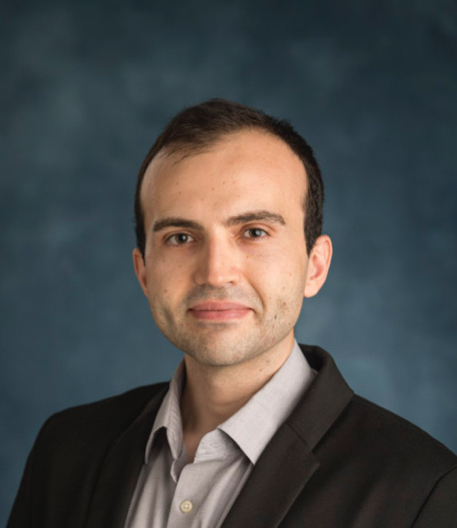
\includegraphics[width=0.2\linewidth]{assets/mert.jpg}
}

\titlegraphic{
\includegraphics[width=0.4\textwidth]{assets/SUSig_2color_Stree_Left.eps}}

\newcommand{\horizontalrule}{
	{
			\vspace{-0.5em}
			\center \rule{\textwidth}{0.1em}
			\vspace{-0.2em}
		}
}

\definecolor{bad}{HTML}{eb6223}
\definecolor{good}{HTML}{9434ed}

\newcommand{\bad}[1]{\textcolor{bad}{#1}}
\newcommand{\good}[1]{\textcolor{good}{#1}}
\newcommand{\purple}[1]{\textcolor{Magenta}{#1}}

% toggle plotting tikz
\def\showtikz{}

%\logo{
\includegraphics[height=0.5cm]{assets/Block_S_2_color.eps}}

%\institute{Stanford University}
\date{}

\begin{document}

\maketitle
%% main content starts %%

\begin{frame}{The Problem}

	{
		\large \bad{Problem}: We don't understand the solution space of
		(even shallow) ReLU networks nearly as well as that of \good{GLMs}.
	}

	\pause
	\vspace{0.5em}
	\horizontalrule
	\vspace{0.5em}

	{
		\large
		Consider the Lasso:
	}

	\pause
	\vspace{0.5em}

	\begin{enumerate}
		\item \textbf{Optimal Sets}: we have an exact \good{polyhedral
			      characterization} and simple criteria for \good{uniqueness}
		      (general position) \citep{tibshirani2013unique}.
		      \pause

		\item \textbf{Regularization Paths}: we know the (min-norm) solution
		      path is \good{continuous} and \good{piece-wise linear}
		      \citep{osborne2000new}.
		      \pause

		\item \textbf{Algorithms}: we have efficient algorithms for
		      \good{homotopy} \citep{efron2004least} and computing \good{minimal
			      solutions} \citep{tibshirani2013unique}.
	\end{enumerate}

\end{frame}

\begin{frame}{Challenges from Non-Convexity}
	\begin{center}
		\Large
		Non-convexity makes extensions beyond GLMs \bad{hard}!
	\end{center}

	\begin{figure}[]
		\centering
		\ifdefined\showtikz
			%! TEX root = ../../main.tex
%% Illustration of step-sizes bound from Armijo line-search. 

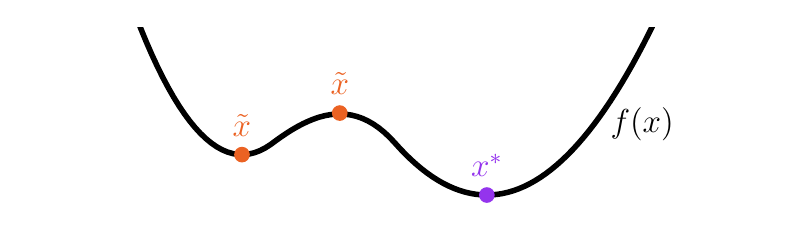
\begin{tikzpicture}[scale=1,
		declare function={
				objective(\x)=      (\x<=-1) * (2*\x*\x + 6*\x + 4)    +
				and(\x>-1, \x<=1) * (\x + 5 - pow(\x,3) - 5*\x*\x) / 4 +
				(\x>1) * (\x*\x - 5*\x + 4);
			}
	]
	\begin{axis}[
			width=0.9\textwidth,
			height=4cm,
			axis x line=none, axis y line=none,
			ymin=-3.25, ymax=5, ytick={-5,...,5}, ylabel=$y$,
			xmin=-5, xmax=7, xtick={-5,...,7}, xlabel=$x$,
		]

		\addplot[name path=function, domain=-3.5:5.23, samples=100, line width=2pt]{objective(x)};

		\node[label={[text=good]90:$x^*$},circle,fill=good,inner sep=2pt] at (axis cs:2.5,-2.25) {};
		\node[label={[text=bad]90:$\tilde x$},circle,fill=bad,inner sep=2pt] at (axis cs:0.09717,1.3) {};
		\node[label={[text=bad]90:$\tilde x$},circle,fill=bad,inner sep=2pt] at (axis cs:-1.5,-0.5) {};

		\node[label={0:$f(x)$}] at (axis cs:4.2,0.8) {};
	\end{axis}
\end{tikzpicture}


		\else
			\Huge Non-Convex Figure
		\fi
	\end{figure}

	\pause
	\begin{itemize}
		\item \textbf{Optimality Conditions}: Stationarity \( \centernot \implies \) optimality.
		      We have no global optimality criteria and no certificates.

		      \vspace{1em}

		      \pause
		\item \textbf{Mathematical Tools}: We lose most of convex analysis
		      and have to work with Clarke stationary points, etc.
		      \vspace{1em}

		      \pause

		\item \textbf{Unintuitive Phenomena}: surprising things happen even
		      with toy neural networks\ldots

	\end{itemize}

\end{frame}

\begin{frame}{Example: Discontinuous Paths}
	Consider training a toy neural network:
	\[
		\min_{w_1} \, \half ((w_1 x_1)_+ - y_1)^2 + \half ((w_1 x_2)_+ - y_2)^2 + \lambda |w_1|.
	\]
	\pause

	\begin{center}
		%! TEX root = ../../main.tex

%% Illustration of cone decomposition. 

\begin{tikzpicture}[scale=1,
		declare function={
				loss(\x)= (4*(\x - 4)^2 + 4)*(x<=4.5) + (8*(\x - 5)^2 + 3)*(x>4.5);
			}
	]
	\begin{axis}[width=\linewidth, height=6cm,
			axis lines=center, yticklabels={,,}, xticklabels={,,},
			ymin=-2, ymax=6, ytick={-2,...,5}, ylabel=$$, x axis line style={-},
				xmin=-6, xmax=6, xtick={-5,...,5}, xlabel=$$, y axis line style={-},
		]

		\addplot[name path=loss, domain=-6:6, samples=200, line width=1pt, color=bad]{loss(x)};

		%% point labels
		% origin point
		\node[circle, fill, inner sep=1pt] at (axis cs:0,0) {};

		% active examples 
		\node[label=right:$(x_1\!\mathbin{,} y_1)$, circle, fill, inner sep=0.5mm] at (axis cs:-5,1) {};
		\node[label=right:$(x_2\!\mathbin{,} y_2)$, circle, fill, inner sep=0.5mm] at (axis cs:0.5,5) {};
	\end{axis}

\end{tikzpicture}%

	\end{center}

	\begin{center}
		\Large
		\textcolor{white}{Goal: Overcome these problems via convexification..}
	\end{center}

\end{frame}

\begin{frame}{Example: Discontinuous Paths}
	Consider training a toy neural network:
	\[
		\min_{w_1} \, \half ((w_1 x_1)_+ - y_1)^2 + \half ((w_1 x_2)_+ - y_2)^2 + \lambda |w_1|.
	\]

	\begin{center}
		%! TEX root = ../../main.tex

%% Illustration of cone decomposition. 

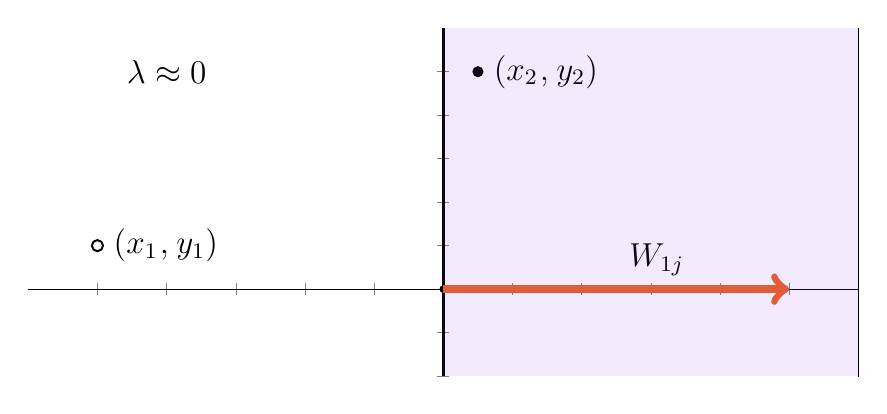
\begin{tikzpicture}[scale=1,
		declare function={
				cone_1(\x)= 10*\x;
				cone_2(\x)= -\x;
				cone_3(\x)= -4*\x;
				bounds(\x)= \x - 10;
			}
	]
	\begin{axis}[width=\linewidth, height=6cm,
			axis lines=center, yticklabels={,,}, xticklabels={,,},
			ymin=-2, ymax=6, ytick={-2,...,5}, ylabel=$$, x axis line style={-},
				xmin=-6, xmax=6, xtick={-5,...,5}, xlabel=$$, y axis line style={-},
		]

		\draw [name path=cone_1, solid, line width=1pt] (axis cs:0,-2) -- (axis cs:0,6);
		\draw [name path=bounds, line width=0pt] (axis cs:6,-2) -- (axis cs:6,6);
		\tikzfillbetween[of=cone_1 and bounds, on layer=ft]{good, opacity=0.1};

		%% point labels
		% origin point
		\node[circle, fill, inner sep=1pt] at (axis cs:0,0) {};

		% active examples 
		\node[label=right:$(x_1\!\mathbin{,} y_1)$, circle, draw, line width=0.25mm, inner sep=0.5mm] at (axis cs:-5,1) {};
		\node[label=right:$(x_2\!\mathbin{,} y_2)$, circle, fill, inner sep=0.5mm] at (axis cs:0.5,5) {};


		% lines
		\draw [->, draw=bad, line width = 1mm] (axis cs:0,0) -- (axis cs:5,0) node[midway,above right] {$W_{1j}$};

        \node[] at (axis cs:-4,5) { $ \lambda \approx 0$ };
	\end{axis}

\end{tikzpicture}%

	\end{center}

	\begin{center}
		\Large
		\textcolor{white}{Goal: Overcome these problems via convexification..}
	\end{center}

\end{frame}

\begin{frame}{Example: Discontinuous Paths}
	Consider training a toy neural network:
	\[
		\min_{w_1} \, \half ((w_1 x_1)_+ - y_1)^2 + \half ((w_1 x_2)_+ - y_2)^2 + \lambda |w_1|.
	\]

	\begin{center}
		%! TEX root = ../../main.tex

%% Illustration of cone decomposition. 

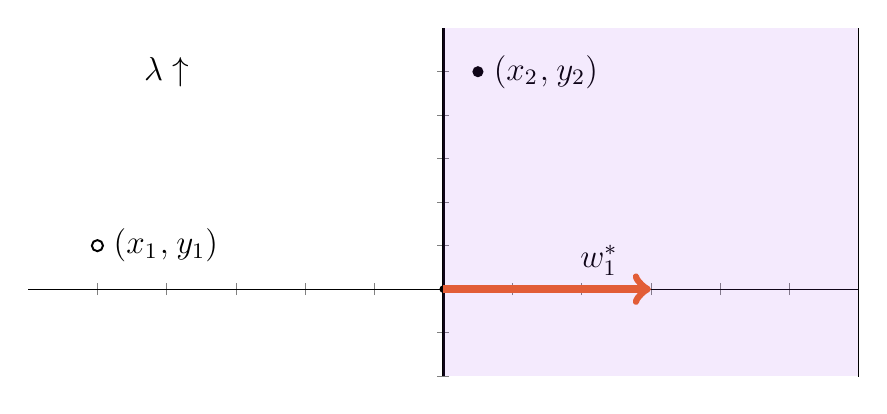
\begin{tikzpicture}[scale=1,
		declare function={
				cone_1(\x)= 10*\x;
				cone_2(\x)= -\x;
				cone_3(\x)= -4*\x;
				bounds(\x)= \x - 10;
			}
	]
	\begin{axis}[width=\linewidth, height=6cm,
			axis lines=center, yticklabels={,,}, xticklabels={,,},
			ymin=-2, ymax=6, ytick={-2,...,5}, ylabel=$$, x axis line style={-},
				xmin=-6, xmax=6, xtick={-5,...,5}, xlabel=$$, y axis line style={-},
		]

		\draw [name path=cone_1, solid, line width=1pt] (axis cs:0,-2) -- (axis cs:0,6);
		\draw [name path=bounds, line width=0pt] (axis cs:6,-2) -- (axis cs:6,6);
		\tikzfillbetween[of=cone_1 and bounds, on layer=ft]{good, opacity=0.1};

		%% point labels
		% origin point
		\node[circle, fill, inner sep=1pt] at (axis cs:0,0) {};

		% active examples 
		\node[label=right:$(x_1\!\mathbin{,} y_1)$, circle, draw, line width=0.25mm, inner sep=0.5mm] at (axis cs:-5,1) {};
		\node[label=right:$(x_2\!\mathbin{,} y_2)$, circle, fill, inner sep=0.5mm] at (axis cs:0.5,5) {};


		% lines
		\draw [->, draw=bad, line width = 1mm] (axis cs:0,0) -- (axis cs:3,0) node[near end,above] {$w^*_{1}$};

        \node[] at (axis cs:-4,5) { $ \lambda \uparrow $ };
	\end{axis}

\end{tikzpicture}%

	\end{center}

	\begin{center}
		\Large
		\textcolor{white}{Goal: Overcome these problems via convexification..}
	\end{center}


\end{frame}

\begin{frame}{Example: Discontinuous Paths}
	Consider training a toy neural network:
	\[
		\min_{w_1} \, \half ((w_1 x_1)_+ - y_1)^2 + \half ((w_1 x_2)_+ - y_2)^2 + \lambda |w_1|.
	\]

	\begin{center}
		%! TEX root = ../../main.tex

%% Illustration of cone decomposition. 

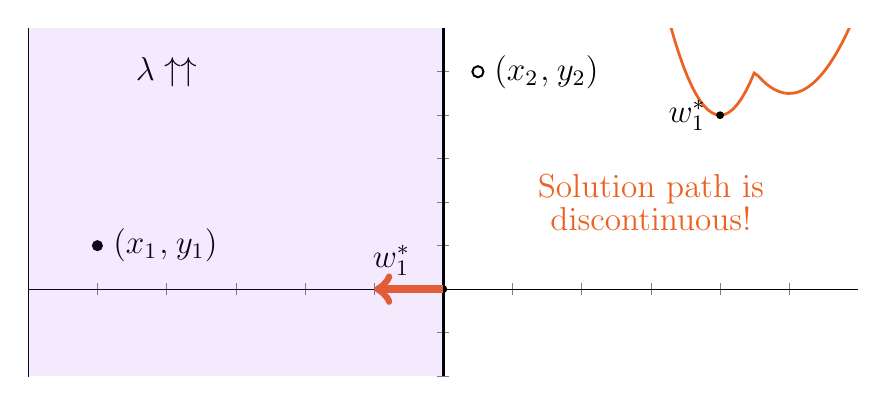
\begin{tikzpicture}[scale=1,
		declare function={
				loss(\x)= (4*(\x - 4)^2 + 4)*(x<=4.5) + (2*(\x - 5)^2 + 4.5)*(x>4.5);
			}
	]
	\begin{axis}[width=\linewidth, height=6cm,
			axis lines=center, yticklabels={,,}, xticklabels={,,},
			ymin=-2, ymax=6, ytick={-2,...,5}, ylabel=$$, x axis line style={-},
				xmin=-6, xmax=6, xtick={-5,...,5}, xlabel=$$, y axis line style={-},
		]
		\addplot[name path=loss, domain=-6:6, samples=200, line width=1pt, color=bad]{loss(x)};
		\node[label=left:$w_1^*$, circle, fill, inner sep=1pt] at (axis cs:4,4) {};

		\draw [name path=cone_1, solid, line width=1pt] (axis cs:0,-2) -- (axis cs:0,6);
		\draw [name path=bounds, line width=0pt] (axis cs:-6,-2) -- (axis cs:-6,6);
		\tikzfillbetween[of=cone_1 and bounds, on layer=ft]{good, opacity=0.1};

		%% point labels
		% origin point
		\node[circle, fill, inner sep=1pt] at (axis cs:0,0) {};

		% active examples 
		\node[label=right:$(x_1\!\mathbin{,} y_1)$, circle, fill, inner sep=0.5mm] at (axis cs:-5,1) {};
		\node[label=right:$(x_2\!\mathbin{,} y_2)$, circle, draw, line width=0.25mm, inner sep=0.5mm] at (axis cs:0.5,5) {};


		% lines
		\draw [->, draw=bad, line width = 1mm] (axis cs:0,0) -- (axis cs:-1,0) node[near end,above] {$w^*_{1}$};

		\node[] at (axis cs:-4,5) { $ \lambda \uparrow \uparrow$ };
    \node[text width=13em, text centered] at (axis cs:3,2) { \bad{Solution path} \bad{is discontinuous!} };
	\end{axis}

\end{tikzpicture}%

	\end{center}

	\pause

	\begin{center}
		\Large
		\good{Goal}: Overcome these problems via convexification.
	\end{center}

\end{frame}

\begin{frame}{Our Contributions}

	{
		\large \good{Overall Approach}: leverage convex reformulations
		of ReLU networks \citep{pilanci2020convex} as an analytical tool.
	}

	\pause
	\vspace{0.5em}
	\horizontalrule
	\vspace{0.5em}

	\begin{enumerate}
		\item \textbf{Optimal Sets}: we characterize all optima of the
		      non-convex training objective.\pause
		      \vspace{0.5em}

		\item \textbf{Uniqueness}: we develop simple criteria for ReLU networks
		      to admit unique solutions up permutation/split symmetries. \pause
		      \vspace{0.5em}

		\item \textbf{Optimal Pruning}: we leverage our theory to give a
		      poly-time procedure for computing minimal ReLU networks.
	\end{enumerate}

\end{frame}


\setbeamercolor{background canvas}{bg=LightCyan}
\begin{frame}{}
	\begin{center}
		\huge I. Background on Convex Reformulations
	\end{center}
\end{frame}
\setbeamercolor{background canvas}{bg=white}

\begin{frame}{Convex Reformulations: Flavor of Results}
	\large

	\textbf{Basic Idea}: We start with a \bad{non-convex} optimization problem and derive
	an equivalent \good{convex} program.

	\pause
	\vspace{2em}

	\textbf{Equivalent} means:
	\vspace{0.5em}
	\begin{itemize}
		\item The global minima have the same values: \( p^* = q^* \)
		      \vspace{0.5em}
		\item We can map every global minimum \( u^* \) for one problem into
		      a global minimum \( v^* \) of the other.
		      \vspace{0.5em}

		      \begin{itemize}
			      \item We call this the \good{solution mapping}.
		      \end{itemize}
	\end{itemize}

\end{frame}


\begin{frame}{Convex Reformulations: Two-Layer ReLU Networks}

	{\large \bad{Non-Convex Problem} (NC-ReLU)}
	\[
		\min_{W_1, w_2} \underbrace{\half \norm{\sum_{j=1}^m (X W_{1j})_+ w_{2j} - y}_2^2}_{\text{Squared Error}}
		+ \underbrace{\lambda \sum_{j=1}^m \norm{W_{1j}}_2^2 + |w_{2j}|^2}_{\text{Weight Decay}},
	\]
	where \( \rbr{x}_+ = \max\cbr{x, 0} \) is the ReLU activation.
	\pause

	\begin{figure}[]
		\centering
		\ifdefined\showtikz
			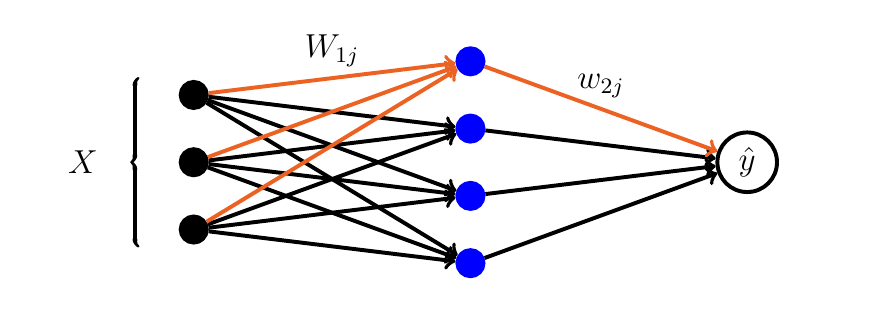
\begin{tikzpicture}[scale=1,
	]
	\begin{axis}[width=\linewidth, height=5cm,
			axis lines=none,  % don't print axis lines
			yticklabels={,,}, xticklabels={,,},
			ymin=0, ymax=8, y axis line style={-},
			xmin=0, xmax=15, x axis line style={-},
		]
		\node [] (input) at (axis cs:1,4) {$X$};
		\node [Input] (input1) at (axis cs:3,2) {};
		\node [Input] (input2) at (axis cs:3,4) {};
		\node [Input] (input3) at (axis cs:3,6) {};

		\draw [decorate, line width = 0.6mm,
			decoration = {calligraphic brace}] (axis cs:2,1.5) --  (axis cs:2,6.5);

		\node [Hidden] (hidden1) at (axis cs:8,1) {};
		\node [Hidden] (hidden2) at (axis cs:8,3) {};
		\node [Hidden] (hidden3) at (axis cs:8,5) {};
		\node [Hidden] (hidden4) at (axis cs:8,7) {};

		\draw [->, style=arrow, draw=black] (input1) -- (hidden1);
		\draw [->, style=arrow, draw=black] (input2) -- (hidden1);
		\draw [->, style=arrow, draw=black] (input3) -- (hidden1);

		\draw [->, style=arrow, draw=black] (input1) -- (hidden2);
		\draw [->, style=arrow, draw=black] (input2) -- (hidden2);
		\draw [->, style=arrow, draw=black] (input3) -- (hidden2);

		\draw [->, style=arrow, draw=black] (input1) -- (hidden3);
		\draw [->, style=arrow, draw=black] (input2) -- (hidden3);
		\draw [->, style=arrow, draw=black] (input3) -- (hidden3);

		\draw [->, style=arrow, draw=bad] (input1) -- (hidden4);
		\draw [->, style=arrow, draw=bad] (input2) -- (hidden4);
		\draw [->, style=arrow, draw=bad] (input3) -- (hidden4) node[pos=0.5,above] {$W_{1j}$};

		\node [Output] (output) at (axis cs:13,4) {$\hat y$};

		\draw [->, style=arrow, draw=black] (hidden1) -- (output);
		\draw [->, style=arrow, draw=black] (hidden2) -- (output);
		\draw [->, style=arrow, draw=black] (hidden3) -- (output);
		\draw [->, style=arrow, draw=bad] (hidden4) -- (output) node[pos=0.5,above] {$w_{2j}$};
	\end{axis}

\end{tikzpicture}%

%\begin{tikzpicture}[scale=1,
%    ]
%    \begin{axis}[width=1.1\linewidth, height=5cm,
%            axis lines=none,  % don't print axis lines
%            yticklabels={,,}, xticklabels={,,},
%            ymin=-0.2, ymax=10.2, x axis line style={-},
%            xmin=-0.2, xmax=20.2, y axis line style={-},
%        ]

%        \filldraw[color=blue!60, fill=blue!5, line width=0.4mm](axis cs:0,5.8) rectangle (axis cs:20, 10);
%        \filldraw[color=red!60, fill=red!5, line width=0.4mm](axis cs:0,0) rectangle (axis cs:20, 4.2);

%        % non-convex models
%        \filldraw[line width=0.4mm, fill=white](axis cs:1,1) rectangle (axis cs:8, 3.2) node[pos=.5] {NC-GReLU};
%        \filldraw[line width=0.4mm, fill=white](axis cs:12,1) rectangle (axis cs:19, 3.2) node[pos=.5] {NC-ReLU};

%        % convex models
%        \filldraw[line width=0.4mm, fill=white](axis cs:1,6.8) rectangle (axis cs:8, 9) node[pos=.5] {C-GReLU};
%        \filldraw[line width=0.4mm, fill=white](axis cs:12,6.8) rectangle (axis cs:19, 9) node[pos=.5] {C-ReLU};

%        \draw [<->, solid, draw=black, line width = 0.6mm] (axis cs:4.5,3.2) -- (axis cs:4.5,6.8) node[right, pos=0.5] {\small Sol. Map};

%        \draw [<->, solid, draw=black, line width = 0.6mm] (axis cs:15.5,3.2) -- (axis cs:15.5,6.8)  node[right, pos=0.5] {\small Sol. Map};

%        \draw [<-, solid, draw=black, line width = 0.6mm] (axis cs:6,9) -- [bend left=15] (axis cs:14, 9);

%        \draw [->, solid, draw=orange, line width = 0.6mm] (axis cs:8,7.9) -- (axis cs:12,7.9);
%        \node[align=center] at (axis cs:10.1, 7.8) {\small Cone\\ \small Decomp.};
%    \end{axis}

%\end{tikzpicture}%


		\else
			\Huge Neural Network Figure
		\fi
	\end{figure}

\end{frame}


\begin{frame}{Aside: ReLU Activation Patterns}

	Each ReLU neuron is active on a half-space:

	\pause

	\begin{figure}[]
		\centering
		\ifdefined\showtikz
			%! TEX root = ../../main.tex

%% Illustration of cone decomposition. 

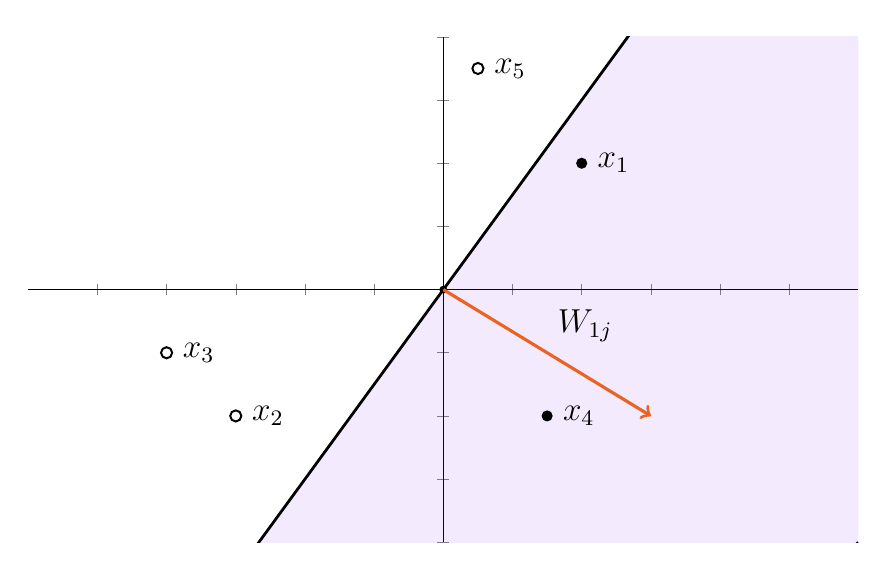
\begin{tikzpicture}[scale=1,
		declare function={
				cone_1(\x)= 3*\x/2;
				cone_2(\x)= -\x;
				cone_3(\x)= -4*\x;
				bounds(\x)= \x - 10;
			}
	]
	\begin{axis}[width=\linewidth, height=8cm,
			axis lines=center, yticklabels={,,}, xticklabels={,,},
			ymin=-4, ymax=4, ytick={-5,...,5}, ylabel=$$, x axis line style={-},
				xmin=-6, xmax=6, xtick={-5,...,5}, xlabel=$$, y axis line style={-},
		]
		\addplot[name path=cone_1, domain=-6:6, samples=100, line width=1pt]{cone_1(x)};
		\addplot[name path=bounds, domain=-6:6, samples=100, line width=1pt]{bounds(x)};

		% add color fill to both cones.

		\addplot fill between[
				of = cone_1 and bounds,
				%split, % calculate segment
				every even segment/.style = {fill=good, fill opacity=0.1},
			];

		%% point labels
		% origin point
		\node[circle, fill, inner sep=1pt] at (axis cs:0,0) {};

		% active examples 
		\node[label=right:$x_1$, circle, fill, inner sep=0.5mm] at (axis cs:2,2) {};
		\node[label=right:$x_4$, circle, fill, inner sep=0.5mm] at (axis cs:1.5,-2) {};

		% inactive examples 
		\node[label=right:$x_2$, circle, line width=0.25mm, draw=black, inner sep=0.5mm] at (axis cs:-3,-2) {};
		\node[label=right:$x_3$, circle, line width=0.25mm, draw=black, inner sep=0.5mm] at (axis cs:-4,-1) {};
		\node[label=right:$x_5$, circle, line width=0.25mm, draw=black, inner sep=0.5mm] at (axis cs:0.5,3.5) {};


		% lines
		\draw [->, draw=bad, line width = 0.4mm] (axis cs:0,0) -- (axis cs:3,-2) node[midway,above right] {$W_{1j}$};
		%\draw [->, draw=red, line width = 0.4mm] (axis cs:2,-2) -- (axis cs:3,-1) node[midway,below right] {$S_{22} \cdot x_2$};
		%\draw [->, draw=red, line width = 0.4mm] (axis cs:0.5,-2) -- (axis cs:-2.5,-2.75) node[pos=0.9,below right] {$S_{33} \cdot x_3$};
	\end{axis}

\end{tikzpicture}%

		\else
			\Huge activation pattern figure
		\fi
	\end{figure}

	\phantom{
		\textbf{Activation Pattern} satisfies \( D_j X W_{1j} = \rbr{X W_{1j}}_+ \)
	}

\end{frame}

\begin{frame}{Aside: ReLU Activation Patterns}

	Each ReLU neuron is active on a half-space:

	\begin{figure}[]
		\centering
		\ifdefined\showtikz
			%! TEX root = ../../main.tex

%% Illustration of cone decomposition. 

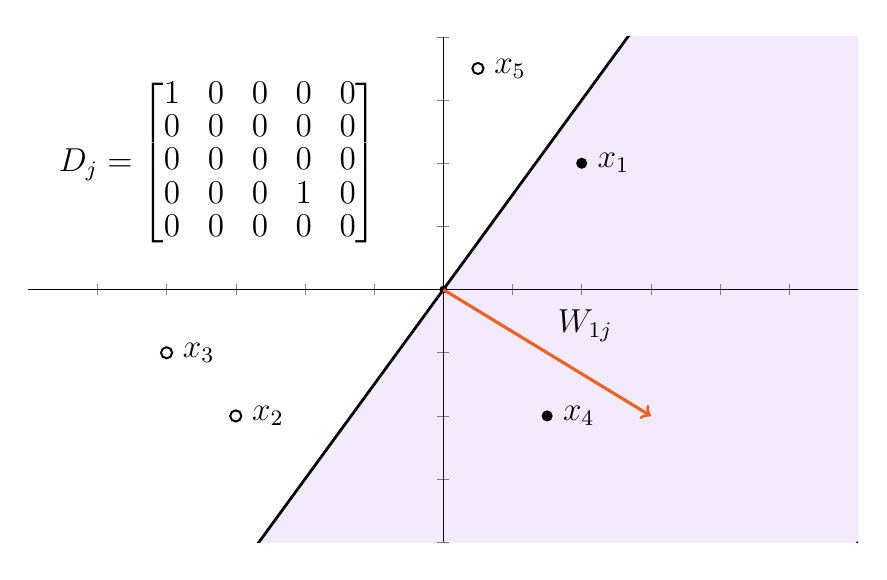
\begin{tikzpicture}[scale=1,
		declare function={
				cone_1(\x)= 3*\x/2;
				cone_2(\x)= -\x;
				cone_3(\x)= -4*\x;
				bounds(\x)= \x - 10;
			}
	]
	\begin{axis}[width=\linewidth, height=8cm,
			axis lines=center, yticklabels={,,}, xticklabels={,,},
			ymin=-4, ymax=4, ytick={-5,...,5}, ylabel=$$, x axis line style={-},
				xmin=-6, xmax=6, xtick={-5,...,5}, xlabel=$$, y axis line style={-},
		]
		\addplot[name path=cone_1, domain=-6:6, samples=100, line width=1pt]{cone_1(x)};
		\addplot[name path=bounds, domain=-6:6, samples=100, line width=1pt]{bounds(x)};

		% add color fill to both cones.

		\addplot fill between[
				of = cone_1 and bounds,
				%split, % calculate segment
				every even segment/.style = {fill=good, fill opacity=0.1},
			];

		%% point labels
		% origin point
		\node[circle, fill, inner sep=1pt] at (axis cs:0,0) {};

		% active examples 
		\node[label=right:$x_1$, circle, fill, inner sep=0.5mm] at (axis cs:2,2) {};
		\node[label=right:$x_4$, circle, fill, inner sep=0.5mm] at (axis cs:1.5,-2) {};

		% inactive examples 
		\node[label=right:$x_2$, circle, line width=0.25mm, draw=black, inner sep=0.5mm] at (axis cs:-3,-2) {};
		\node[label=right:$x_3$, circle, line width=0.25mm, draw=black, inner sep=0.5mm] at (axis cs:-4,-1) {};
		\node[label=right:$x_5$, circle, line width=0.25mm, draw=black, inner sep=0.5mm] at (axis cs:0.5,3.5) {};


		% activation pattern
		\node[] at (axis cs:-3.25,2) {
			$D_j = \begin{bmatrix}
					1 & 0 & 0 & 0 & 0 \\
					0 & 0 & 0 & 0 & 0 \\
					0 & 0 & 0 & 0 & 0 \\
					0 & 0 & 0 & 1 & 0 \\
					0 & 0 & 0 & 0 & 0 \\
				\end{bmatrix}
			$};

		% lines
		\draw [->, draw=bad, line width = 0.4mm] (axis cs:0,0) -- (axis cs:3,-2) node[midway,above right] {$W_{1j}$};
		%\draw [->, draw=red, line width = 0.4mm] (axis cs:2,-2) -- (axis cs:3,-1) node[midway,below right] {$S_{22} \cdot x_2$};
		%\draw [->, draw=red, line width = 0.4mm] (axis cs:0.5,-2) -- (axis cs:-2.5,-2.75) node[pos=0.9,below right] {$S_{33} \cdot x_3$};
	\end{axis}

\end{tikzpicture}%

		\else
			\Huge activation pattern figure
		\fi
	\end{figure}

	\pause
	\textbf{Activation Pattern} satisfies \( D_j X W_{1j} = \rbr{X W_{1j}}_+ \)

\end{frame}

\begin{frame}{Aside: ReLU Activation Patterns}

	Each ReLU neuron is active on a half-space:

	\begin{figure}[]
		\centering
		\ifdefined\showtikz
			%! TEX root = ../../main.tex

%% Illustration of cone decomposition. 

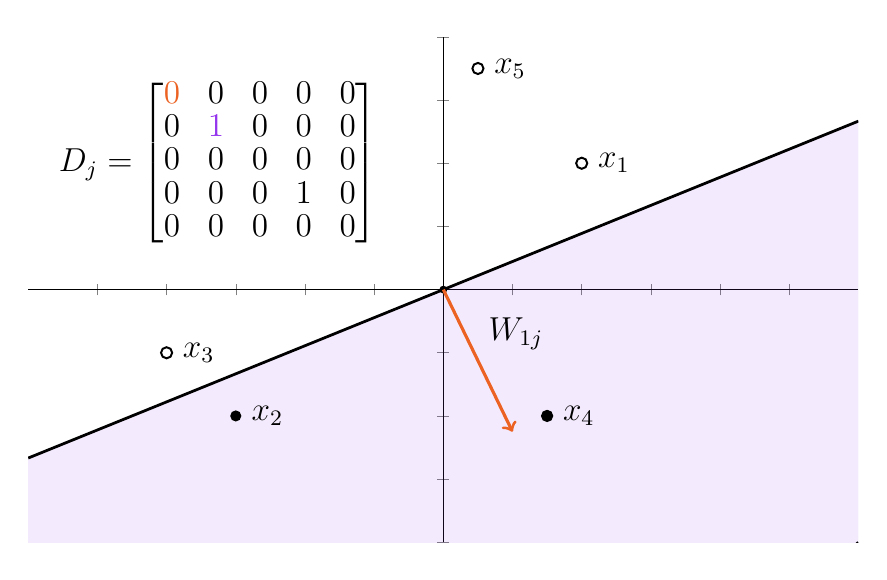
\begin{tikzpicture}[scale=1,
		declare function={
				cone_1(\x)= \x/2.25;
				cone_2(\x)= -\x;
				cone_3(\x)= -4*\x;
				bounds(\x)= \x - 10;
			}
	]
	\begin{axis}[width=\linewidth, height=8cm,
			axis lines=center, yticklabels={,,}, xticklabels={,,},
			ymin=-4, ymax=4, ytick={-5,...,5}, ylabel=$$, x axis line style={-},
				xmin=-6, xmax=6, xtick={-5,...,5}, xlabel=$$, y axis line style={-},
		]
		\addplot[name path=cone_1, domain=-6:6, samples=100, line width=1pt]{cone_1(x)};
		\addplot[name path=bounds, domain=-6:6, samples=100, line width=1pt]{bounds(x)};

		% add color fill to both cones.

		\addplot fill between[
				of = cone_1 and bounds,
				%split, % calculate segment
				every even segment/.style = {fill=good, fill opacity=0.1},
			];

		%% point labels
		% origin point
		\node[circle, fill, inner sep=1pt] at (axis cs:0,0) {};

		% active examples 
		\node[label=right:$x_1$, circle, line width=0.25mm, draw=black, inner sep=0.5mm] at (axis cs:2,2) {};
		\node[label=right:$x_4$, circle, fill, draw=black, inner sep=0.5mm] at (axis cs:1.5,-2) {};

		% inactive examples 
		\node[label=right:$x_2$, circle, fill, inner sep=0.5mm] at (axis cs:-3,-2) {};
		\node[label=right:$x_3$, circle, line width=0.25mm, draw=black, inner sep=0.5mm] at (axis cs:-4,-1) {};
		\node[label=right:$x_5$, circle, line width=0.25mm, draw=black, inner sep=0.5mm] at (axis cs:0.5,3.5) {};


		% activation pattern
		\node[] at (axis cs:-3.25,2) {
			$D_j = \begin{bmatrix}
					\bad{0} & 0        & 0 & 0 & 0 \\
					0       & \good{1} & 0 & 0 & 0 \\
					0       & 0        & 0 & 0 & 0 \\
					0       & 0        & 0 & 1 & 0 \\
					0       & 0        & 0 & 0 & 0 \\
				\end{bmatrix}
			$};

		% lines
		\draw [->, draw=bad, line width = 0.4mm] (axis cs:0,0) -- (axis cs:1,-2.25) node[midway,above right] {$W_{1j}$};

	\end{axis}

\end{tikzpicture}%

		\else
			\Huge activation pattern figure
		\fi
	\end{figure}


	\textbf{Activation Pattern} satisfies \( D_j X W_{1j} = \rbr{X W_{1j}}_+ \)

\end{frame}


\begin{frame}{Convex Reformulations: Convex Problem}

	{\large \good{Convex Reformulation} (C-ReLU)} \citep{pilanci2020convex}
	\[
		\begin{aligned}
			\min_{v, w} & \half \norm{\sum_{j=1}^p D_j X (v_j - w_j) - y}_2^2 +
			\lambda \sum_{j=1}^p \norm{v_j}_2 + \norm{w_j}_2                    \\
			            & \hspace{0.2em} \text{s.t. }
			v_j, w_j \in \calK_j := \cbr{w : (2D_j - I) X w \geq 0},
		\end{aligned}
	\]
	where \( D_j = \text{diag}[\mathbbm{1}(X g_j \geq 0)] \).
	\pause

	\begin{figure}[]
		\centering
		\ifdefined\showtikz
			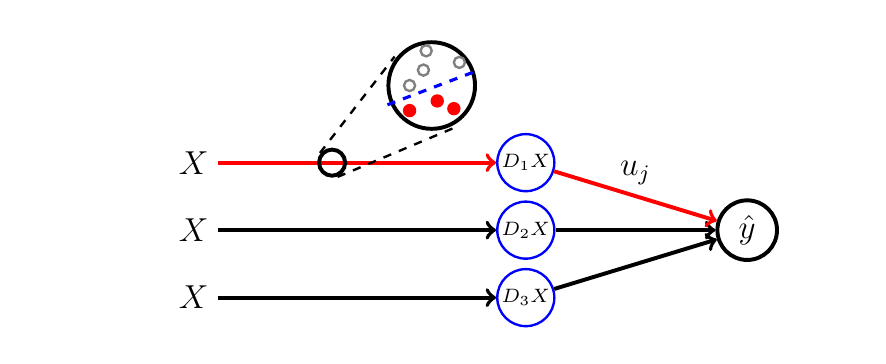
\begin{tikzpicture}[scale=1,
	]
	\begin{axis}[width=\linewidth, height=5.5cm,
			axis lines=none,  % don't print axis lines
			yticklabels={,,}, xticklabels={,,},
			ymin=0, ymax=8, y axis line style={-},
			xmin=0, xmax=15, x axis line style={-},
		]
		\node [] (input1) at (axis cs:3,1) {$X$};
		\node [] (input2) at (axis cs:3,2.75) {$X$};
		\node [] (input3) at (axis cs:3,4.5) {$X$};

        \node [Splits] (hidden1) at (axis cs:9,1) {\scriptsize $D_3 X$};
		\node [Splits] (hidden2) at (axis cs:9,2.75) {\scriptsize $D_2 X$};
		\node [Splits] (hidden3) at (axis cs:9,4.5) {\scriptsize $D_1 X$};

		\draw [->, style=arrow, draw=black] (input1) -- (hidden1);

		\draw [->, style=arrow, draw=black] (input2) -- (hidden2);

		\draw [->, style=arrow, draw=red] (input3) -- (hidden3);

		\node [Output] (output) at (axis cs:13,2.75) {$\hat y$};

		\draw [->, style=arrow, draw=black] (hidden1) -- (output);
		\draw [->, style=arrow, draw=black] (hidden2) -- (output);
		\draw [->, style=arrow, draw=red] (hidden3) -- (output) node[pos=0.5,above] {$u_j$};

		\draw [draw=black, line width=0.3mm, dashed] (axis cs:5.6, 4.13) -- (axis cs:7.7,5.4);
		\draw [draw=black, line width=0.3mm, dashed] (axis cs:5.28, 4.75) -- (axis cs:6.63,7.25);

		\node [draw=black, minimum size=0.3cm, shape=circle, solid, line width=0.5mm] (examine) at (axis cs:5.5,4.5) {};
		\node [draw=black, minimum size=1.1cm, shape=circle, solid, line width=0.5mm] (closeup) at (axis cs:7.3,6.5) {};

		\node [fill=white, draw=gray, line width=0.3mm, inner sep=0.05cm, shape=circle] at (axis cs:7.8,7.1) {};
		\node [fill=white, draw=gray, line width=0.3mm, inner sep=0.05cm, shape=circle] at (axis cs:7.15,6.9) {};
		\node [fill=white, draw=gray, line width=0.3mm, inner sep=0.05cm, shape=circle] at (axis cs:7.2,7.4) {};
		\node [fill=white, draw=gray, line width=0.3mm, inner sep=0.05cm, shape=circle] at (axis cs:6.9,6.5) {};

		\draw [draw=Blue, dashed, line width=0.4mm] (axis cs:6.5,6.) -- (axis cs:8.15,6.9);

		\node [fill=Red, inner sep=0.06cm, shape=circle] at (axis cs:6.9,5.85) {};
		\node [fill=Red, inner sep=0.06cm, shape=circle] at (axis cs:7.4,6.1) {};
		\node [fill=Red, inner sep=0.06cm, shape=circle] at (axis cs:7.7,5.9) {};

	\end{axis}

\end{tikzpicture}%

%\begin{tikzpicture}[scale=1,
%    ]
%    \begin{axis}[width=1.1\linewidth, height=5cm,
%            axis lines=none,  % don't print axis lines
%            yticklabels={,,}, xticklabels={,,},
%            ymin=-0.2, ymax=10.2, x axis line style={-},
%            xmin=-0.2, xmax=20.2, y axis line style={-},
%        ]

%        \filldraw[color=blue!60, fill=blue!5, line width=0.4mm](axis cs:0,5.8) rectangle (axis cs:20, 10);
%        \filldraw[color=red!60, fill=red!5, line width=0.4mm](axis cs:0,0) rectangle (axis cs:20, 4.2);

%        % non-convex models
%        \filldraw[line width=0.4mm, fill=white](axis cs:1,1) rectangle (axis cs:8, 3.2) node[pos=.5] {NC-GReLU};
%        \filldraw[line width=0.4mm, fill=white](axis cs:12,1) rectangle (axis cs:19, 3.2) node[pos=.5] {NC-ReLU};

%        % convex models
%        \filldraw[line width=0.4mm, fill=white](axis cs:1,6.8) rectangle (axis cs:8, 9) node[pos=.5] {C-GReLU};
%        \filldraw[line width=0.4mm, fill=white](axis cs:12,6.8) rectangle (axis cs:19, 9) node[pos=.5] {C-ReLU};

%        \draw [<->, solid, draw=black, line width = 0.6mm] (axis cs:4.5,3.2) -- (axis cs:4.5,6.8) node[right, pos=0.5] {\small Sol. Map};

%        \draw [<->, solid, draw=black, line width = 0.6mm] (axis cs:15.5,3.2) -- (axis cs:15.5,6.8)  node[right, pos=0.5] {\small Sol. Map};

%        \draw [<-, solid, draw=black, line width = 0.6mm] (axis cs:6,9) -- [bend left=15] (axis cs:14, 9);

%        \draw [->, solid, draw=orange, line width = 0.6mm] (axis cs:8,7.9) -- (axis cs:12,7.9);
%        \node[align=center] at (axis cs:10.1, 7.8) {\small Cone\\ \small Decomp.};
%    \end{axis}

%\end{tikzpicture}%


		\else
			\Huge convex reformulation figure
		\fi
	\end{figure}
\end{frame}

\begin{frame}{Convex Reformulations: Hardness}

	\textbf{Result}: if \( m \geq m^* \) for some \( m^* \leq n \),
	then C-ReLU and NC-ReLU are \good{equivalent}
	\citep{pilanci2020convex}.

	\pause
	\horizontalrule

	How ``hard'' is the convex program?
	\pause

	\[
		p = \abs{\cbr{D_j = \text{diag}[\mathbbm{1}(X g_j \geq 0)] : g_j \in \R^d }}
	\]

	\vspace{2em}
	\pause

	The \textbf{convex program} is:
	\vspace{0.5em}
	\begin{itemize}
		\item \bad{Exponential in general}: \( p \in O(r \cdot (\frac{n}{r})^r) \),
		      where \( r = \text{rank}(X) \).
		      \vspace{0.25em}
		      \begin{itemize}
			      \item Bound comes from theory of hyperplane arrangements \citep{winder1966partitions}.
		      \end{itemize}
		      \pause

		      \vspace{0.5em}

		\item Highly \good{structured} --- it's a (constrained) GLM!
	\end{itemize}

	\vspace{1em}
	\pause

	\begin{center}
		\Large
		We exchange one kind of hardness for another.
	\end{center}

\end{frame}

\setbeamercolor{background canvas}{bg=LightCyan}
\begin{frame}{}
	\begin{center}
		\huge II. Optimal Sets
	\end{center}
\end{frame}
\setbeamercolor{background canvas}{bg=white}

\begin{frame}{Characterizing the Optimal Set}

	{
		\large
		{\Large
			Proof Roadmap:
		}
		\vspace{2em}
		\begin{enumerate}
			\large
			\item \pause
			      Characterize solutions to the \good{convex reformulation}
			      using strong duality and KKT conditions.
			      \vspace{1ex}
			      \pause
			\item Extend results to \bad{non-convex} ReLU networks
			      using the solution mapping.
			      \vspace{1ex}
			      \pause
			\item Leverage explicit characterization of the optimal
			      set for \good{new insights and algorithms}.
		\end{enumerate}
	}


\end{frame}

\begin{frame}{Characterizing the Optimal Set}

	{
		\large
		{\Large
			Proof Roadmap:
		}
		\vspace{2em}
		\begin{enumerate}
			\large
			\item \textbf{Characterize solutions to the \good{convex reformulation}
				      using strong duality and KKT conditions.}
			      \vspace{1ex}
			\item Extend results to \bad{non-convex} ReLU networks
			      using the solution mapping.
			      \vspace{1ex}
			\item Leverage explicit characterization of the optimal
			      set for \good{new insights and algorithms}.
		\end{enumerate}
	}

\end{frame}

\begin{frame}{C-ReLU Optimal Set}

	{\raggedright
		\large
		1. Characterize solutions to the \good{convex reformulation}
		using strong duality and KKT conditions.
		\vspace{3ex}
		\pause
	}

	\horizontalrule

	\textbf{C-ReLU Solution Set}:
	\[
		\begin{aligned}
			\solfn(\lambda) & =
			\argmin_{v_i, w_i \in \calK_i} \, \bigg\{
			\half \bigg\|\sum_{D_i \in \tilde \calD} D_i X (v_i - w_i), y\bigg\|_2^2                    \\
			                & \quad \quad + \lambda\sum_{D_i \in \tilde \calD}\norm{v_i}_2+\norm{w_i}_2
			\bigg\}.
		\end{aligned}
	\]

	\pause

	\begin{itemize}
		\item Convex objective + linear constraints \( \implies \) strong duality!
		      \pause
		\item Introduce dual variables \( \rho \) and analyze the KKT conditions.
		      \pause
		\item Define
		      \(
		      \theta =
		      \begin{bmatrix}
			      v_i \\
			      -w_i
		      \end{bmatrix}
		      \)
		      and index \( D_i \)'s from \( 1 \) to \( 2p \).

	\end{itemize}

\end{frame}

\begin{frame}{C-ReLU Optimality Conditions}

	We form the Lagrangian for the convex reformulation:

	\begin{equation*}
		\begin{aligned}
			\calL(\theta, \rho)
			 & = \half \norm{\sum_{i=1}^{2p} D_i X \theta_i - y}_2^2
			+ \lambda\sum_{i=1}^{2p}\norm{\theta_i}_2
			- \sum_{i=1}^{2p} \abr{K_i^\top \rho, \theta_i},
		\end{aligned}
	\end{equation*}
	where \( K_{i} = (2D_i - I) X \).

	\pause
	\horizontalrule

	The \good{KKT conditions} are necessary and sufficient for optimality:\pause

	\vspace{1ex}
	\begin{itemize}
		\item Define the \textbf{optimal model fit}: \( \hat y = \sum_{i=1}^{2p} D_i X \theta_i  \).
		      \pause
		\item Stationarity of the Lagrangian:
		      \[
			      \underbrace{X^\top D_i (\hat y - y) + K_i^\top \ri}_{q_i}
			      \in \bad{\partial \lambda \norm{\theta_i}_2}.
		      \]
		      \pause
		\item It turns out each ``block correlation'' \( q_i \) is \good{unique} WLOG!
	\end{itemize}

\end{frame}

\begin{frame}{Characterizing the Optimal Set}

	\textbf{Stationary Lagrangian}:
	\[
		X^\top D_i (\hat y - y) + K_i^\top \ri =:
		\bad{q_i \in \partial \lambda \norm{\theta_i}_2}.
	\]

	\pause
	\horizontalrule

	\textbf{Non-zero Blocks}:
	\begin{itemize}
		\item Suppose \( \good{\theta_i \neq 0} \).
		      \pause
		\item Then \(  \nabla_\theta \lambda \norm{\theta_i}_2
		      = \lambda \frac{\theta_i}{\norm{\theta_i}_2} \) and
		\item There exists some \( \alpha_\bi > 0 \) for which,
		      \[
			      q_i = \lambda \frac{\theta_i}{\norm{\theta_i}_2}
			      \implies \theta_i = \good{\alpha_\bi} q_i.
		      \]
		      \pause
		      \vspace{-1em}
		\item Every optimal \( \theta_i^* \neq 0 \) is collinear with the
		      (unique) \( q_i \) vector.
	\end{itemize}

\end{frame}

\begin{frame}{C-ReLU: the Optimal Set}
	\vspace{-2ex}
	\begin{itemize}
		\item
		      \textbf{Optimal Fit: }       \( \hat y = \sum_{i=1}^{2p} D_i X \theta_i  \).
		      \vspace{1ex}

		\item
		      \textbf{Block Correlation: } \( q_i := X^\top D_i (\hat y - y) + K_i^\top \ri \).
		      \pause
		      \vspace{1ex}

		\item
		      \textbf{Support Set: }      \( \calS_\lambda
		      = \cbr{\bi \in [2p] : \exists \theta \in \solfn(\lambda), \
			      \theta_i \neq 0} \).
	\end{itemize}

	\vspace{-2ex}
	\pause
	\horizontalrule
	\vspace{-1ex}

	\begin{proposition}[Informal]
		Fix \( \lambda > 0 \).
		The optimal set of the C-ReLU problem is
		given by
		\begin{equation*}
			\begin{aligned}
				\solfn(\lambda) =
				\big\{ & \theta  :
				\forall \, \bi  \in  \calS_\lambda,
				\good{\theta_i =  \alpha_\bi q_i}, \alpha_\bi \geq 0, \,      \\
				       & \quad \forall \, j \in [2p] \setminus \calS_\lambda,
				\theta_{j} = 0, \, \good{\sum_{i=1}^{2p} D_i X \theta_i = \hat y}
				\big\}
			\end{aligned}
		\end{equation*}
	\end{proposition}

\end{frame}

\begin{frame}{Returning to our Roadmap}

	{
		\large
		{\Large
			Proof Roadmap:
		}
		\pause
		\vspace{2em}
		\begin{enumerate}
			\large
			\item Characterize solutions to the \good{convex reformulation}
			      using strong duality and KKT conditions.
			      \vspace{1ex}
			\item \textbf{Extend results to \bad{non-convex} ReLU networks
				      using the solution mapping.}
			      \vspace{1ex}
			\item Leverage explicit characterization of the optimal
			      set for \good{new insights and algorithms}.
		\end{enumerate}
	}

\end{frame}


\begin{frame}{C-ReLU: Mapping back to Non-Convex Networks}

	{\raggedright
		\large
		2. Extend results to \bad{non-convex} ReLU networks
		using the solution mapping.
		\pause
	}
	\horizontalrule

	We need to do some accounting for \bad{model symmetries}:
	\pause
	\begin{itemize}
		\item \textbf{Permutations}: Re-ordering neurons (i.e. permutations).
		      \pause

		\item \textbf{Splits}: Splitting a neuron into two collinear neurons.
		      \pause
	\end{itemize}


	\begin{theorem}[Informal]
		Suppose \( m \geq m^* \).
		Then the optimal set for NC-ReLU up to
		\bad{permutation/split symmetries} is
		\vspace{-1ex}
		\begin{equation*}
			\begin{aligned}
				\hspace{-0.5em} \calO_\lambda  = \,
				\big\{
				 & (W_1,  w_2) :
				\, f_{W_1, w_2}(X)  =  \hat y,                       \\
				 & \forall \, \bi  \in  \calS_\lambda,
				W_{1i} = (\sfrac{\alpha_{i}}{\lambda})^{\sfrac{1}{2}} q_i,
				w_{2i} = (\alpha_i \lambda)^{\sfrac{1}{2}},
				\alpha_i \geq 0                                      \\
				 & \forall \, \bi  \in [2p] \setminus \calS_\lambda,
				W_{1i} = 0, \, w_{2i} = 0
				\big\}.
			\end{aligned}
		\end{equation*}
	\end{theorem}

\end{frame}

\begin{frame}{C-ReLU: Appearance of Solution Sets}
	\begin{figure}[]
		\centering
		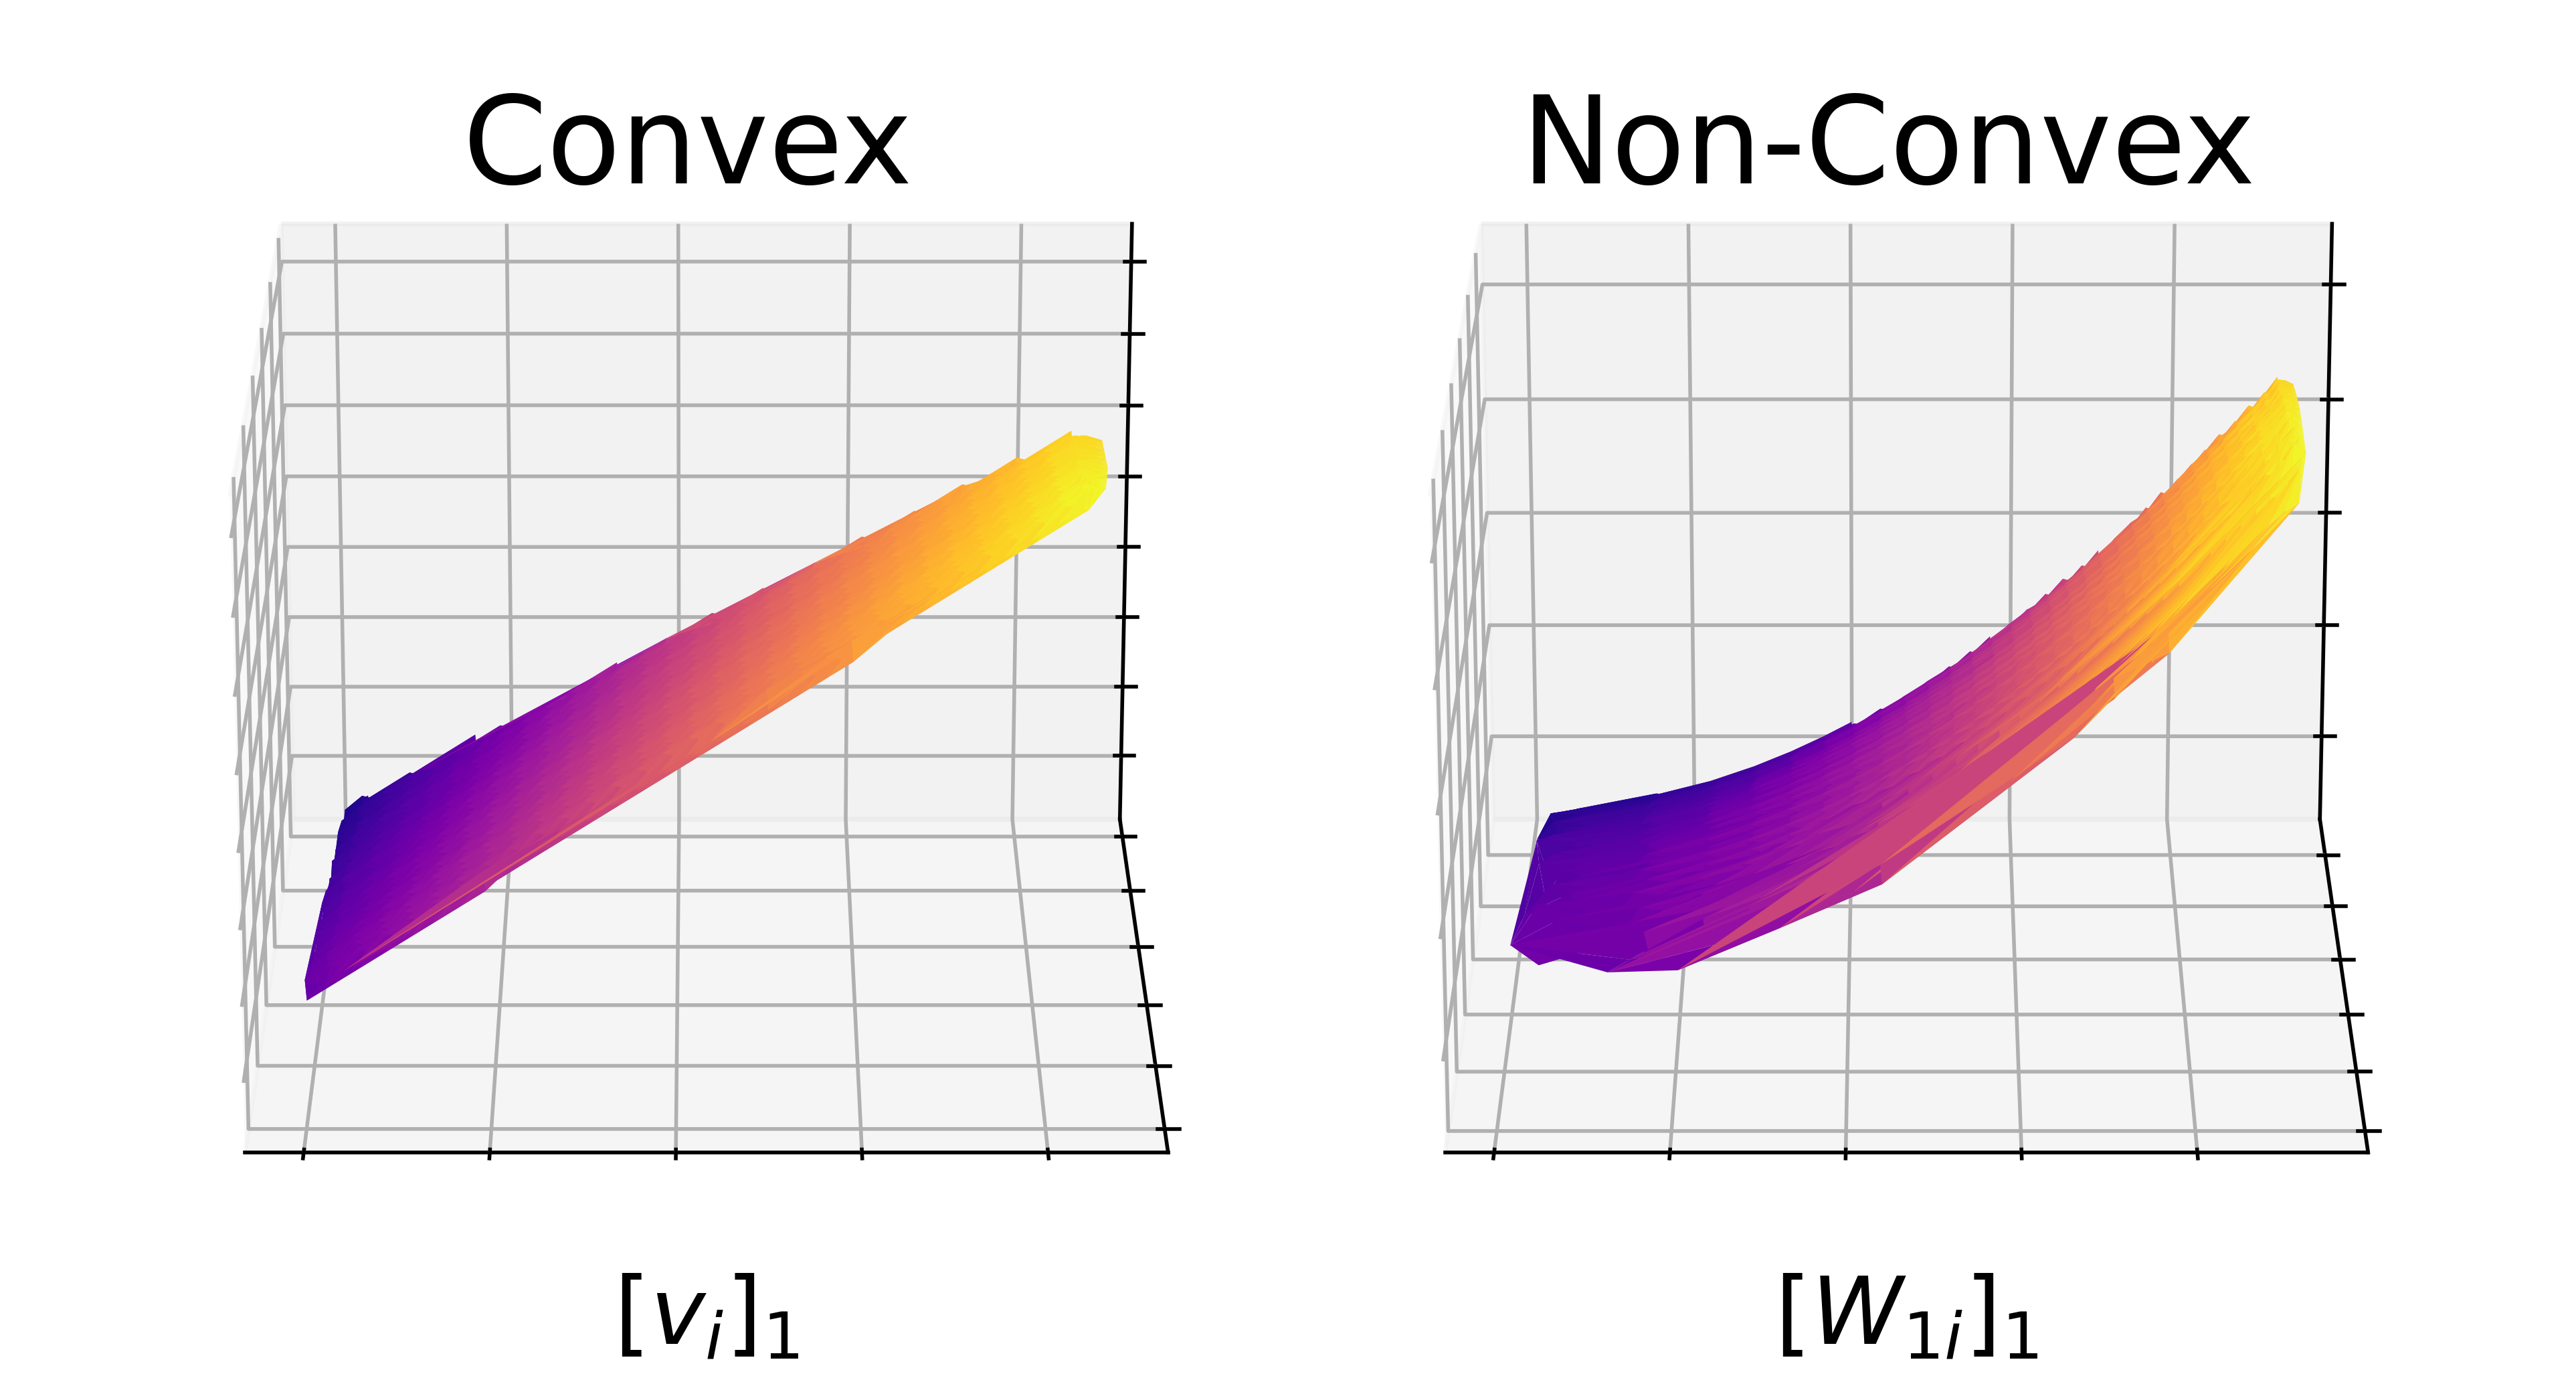
\includegraphics[width=0.96\textwidth]{assets/solution_sets_vis_270.png}
	\end{figure}

	\begin{itemize}
		\item The non-convex parameterization maps the \good{convex polytope} of
		      solutions into a \bad{curved manifold}.
	\end{itemize}


\end{frame}


\begin{frame}{Exploring the Optimal Set}

	\begin{figure}[t]
		\centering
		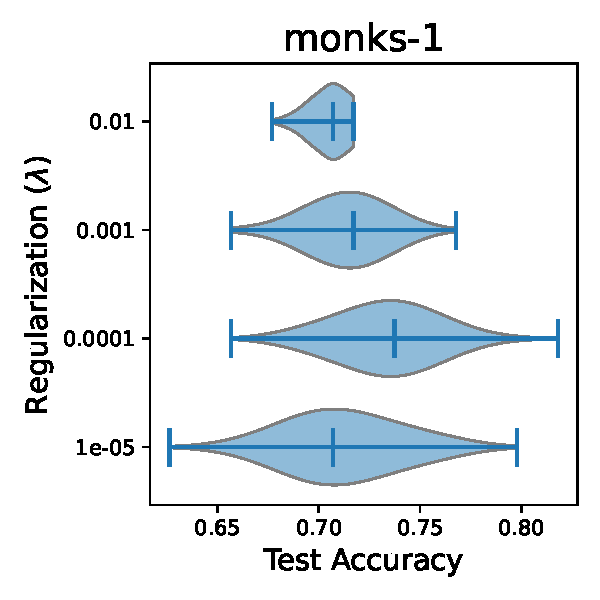
\includegraphics[width=0.48\linewidth]{assets/dist_paper_monks-1.pdf}
		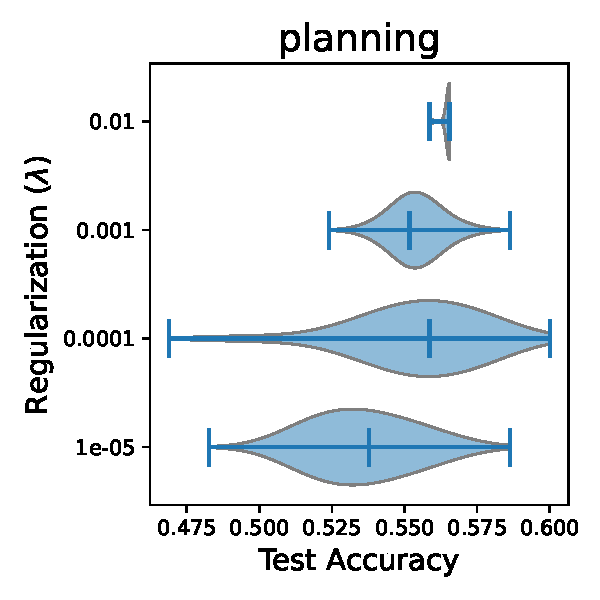
\includegraphics[width=0.48\linewidth]{assets/dist_paper_planning.pdf}
	\end{figure}
	\begin{itemize}
		\item Take 10,000 samples from the set of optimal neural networks.
		\item All samples have (i) \textbf{same training accuracy},
		      (ii)~\textbf{same model norm}, but generalize very differently.
	\end{itemize}
\end{frame}


\setbeamercolor{background canvas}{bg=LightCyan}

\begin{frame}{}
	\begin{center}
		\huge III. Pruning
	\end{center}
\end{frame}
\setbeamercolor{background canvas}{bg=white}


\begin{frame}{Leveraging our Characterization}

	{\Large Proof Roadmap:}
	\vspace{2em}
	\pause

	\begin{enumerate}
		\large
		\item Characterize solutions to the \good{convex reformulation}
		      using strong duality and KKT conditions.
		      \vspace{1ex}

		\item Extend results to \bad{non-convex} ReLU networks
		      using the solution mapping.
		      \vspace{1ex}

		\item \textbf{Leverage explicit characterization of the optimal
			      set for \good{new insights and algorithms}.}
	\end{enumerate}
\end{frame}

\begin{frame}{Optimal Pruning: Polytope of Solutions}

	{\raggedright
		\large
		3. Leverage explicit characterization of the optimal
		set for \good{new insights and algorithms}.
		\pause
	}

	\horizontalrule

	\begin{columns}
		\begin{column}{0.5\textwidth}

			\begin{equation*}
				\begin{aligned}
					 & \solfn(\lambda) =
					\big\{ \theta  : \sum_{i=1}^{2p} D_i X \theta_i = \hat y,      \\
					 & \hspace{5em} \forall \, \bi  \in  \calS_\lambda,
					\theta_i =  \alpha_\bi q_i, \alpha_\bi \geq 0, \,              \\
					 & \hspace{5em} \forall \, j \in [2p] \setminus \calS_\lambda,
					\theta_{j} = 0
					\big\}
				\end{aligned}
			\end{equation*}

			\pause
			The C-ReLU optimal set is a \good{convex polytope}.

		\end{column}
		\begin{column}{0.5\textwidth}
			\pause
			\begin{figure}[c]
				\centering
				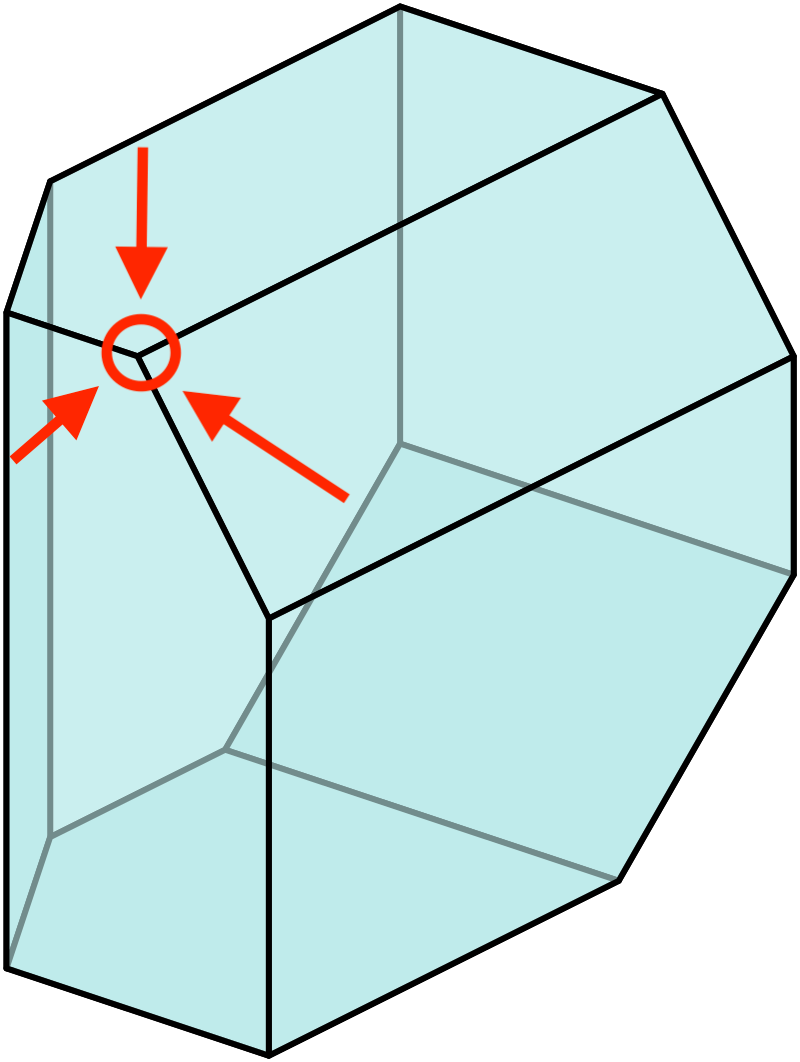
\includegraphics[width=0.8\textwidth]{assets/polytope.png}
				\caption{}
				\label{fig:}
			\end{figure}
		\end{column}
	\end{columns}

\end{frame}

\begin{frame}{Optimal Pruning: Vertices}

	\begin{enumerate}
		\item
		      Stack the \( q_i \) vectors into a matrix \( Q =
		      \begin{bmatrix}
			      \vert &        & \vert  \\
			      q_1   & \cdots & q_{2p} \\
			      \vert &        & \vert  \\
		      \end{bmatrix}.
		      \)

		      \pause
		\item
		      The C-ReLU Optimal Set in \( \alpha \) space is then,
		      \begin{equation}
			      \begin{aligned}
				      \solfn(\lambda) & =
				      Q_{\calS_\lambda} \big\{ \alpha \succeq 0  :
				      \sum_{i \in \calS_\lambda} (D_i X q_i) \alpha_i = \hat y,
				      \big\}                                                       \\
				                      & = Q_{\calS_\lambda} \calP_{\calS_\lambda}.
			      \end{aligned}
		      \end{equation}

		      \pause

		\item \( \bar \alpha \in \calP_{\calS_\lambda} \) is a \good{vertex}
		      iff \( \cbr{D_i X q_i}_{\bar \alpha_i \neq 0} \) are linearly independent.
	\end{enumerate}

	\pause
	\horizontalrule

	{\large Are these vertices \good{special} in some way?}

\end{frame}

\begin{frame}{Optimal Pruning: Algorithm}
	\textbf{Definition}: A optimal C-ReLU model \( \theta^* \) is minimal
	if there does
	not exist another optimal model \( \theta' \) with strictly smaller support.

	\vspace{3ex}
	\pause

	\begin{beamercolorbox}[wd=\textwidth,sep=1em]{result}
		\textbf{Proposition 3.2} (informal):
		For \( \lambda > 0 \), \( \theta \in \solfn(\lambda) \) is \good{minimal}
		iff
		the vectors \( \cbr{D_i X q_i}_{\alpha_i \neq 0} \)
		are linearly independent.
	\end{beamercolorbox}

	\vspace{3ex}
	\pause

	\textbf{We prove}:
	\begin{itemize}
		\item Vertices of \( \solfn(\lambda) \) are minimal models.
		      \pause
		\item There are at most \( n \) neurons in a minimal model.
		      \pause
		\item Pruning from any optimal model will give a minimal model.
	\end{itemize}

\end{frame}

\begin{frame}{Optimal Pruning: Pseudo-code}
	\begin{algorithm}[H]
		\caption{Pruning solutions}
		\begin{algorithmic}
			\STATE {\bfseries Input:} data matrix \( X \), solution \( \theta \).
			\STATE \( k \gets 0 \).
			\STATE \( \theta^k \gets \theta \).
			\WHILE {\( \exists \beta \neq 0 \) s.t. \( \good{\sum_{\bi \in \act(\theta^k)} \beta_\bi D_i X \theta_i^k = 0} \)}
			\STATE \( \bi^k \gets \argmax_{\bi} \cbr{|\beta_\bi| : \bi \in \act(\theta^k)}  \)
			\STATE \( t^k \gets 1/|\beta_{\bi^k}| \)
			\STATE \( \theta^{k+1} \gets \theta^k (1 - t^k \beta_\bi) \)
			\STATE \( k \gets k + 1 \)
			\ENDWHILE
			\STATE {\bfseries Output:} final weights \( \theta^k \)
		\end{algorithmic}
	\end{algorithm}

	\pause

	Let \( r = \text{rank}(X) \). Complexity to compute a minimal model:

	\[ O\rbr{d^3 r^3 (\frac{n}{r})^{3r} + \good{(n^3 + nd) r (\frac{n}{r})^r}}. \]

\end{frame}


\begin{frame}{(Sub)-Optimal Pruning on UCI}
	\begin{figure}[t]
		\centering
		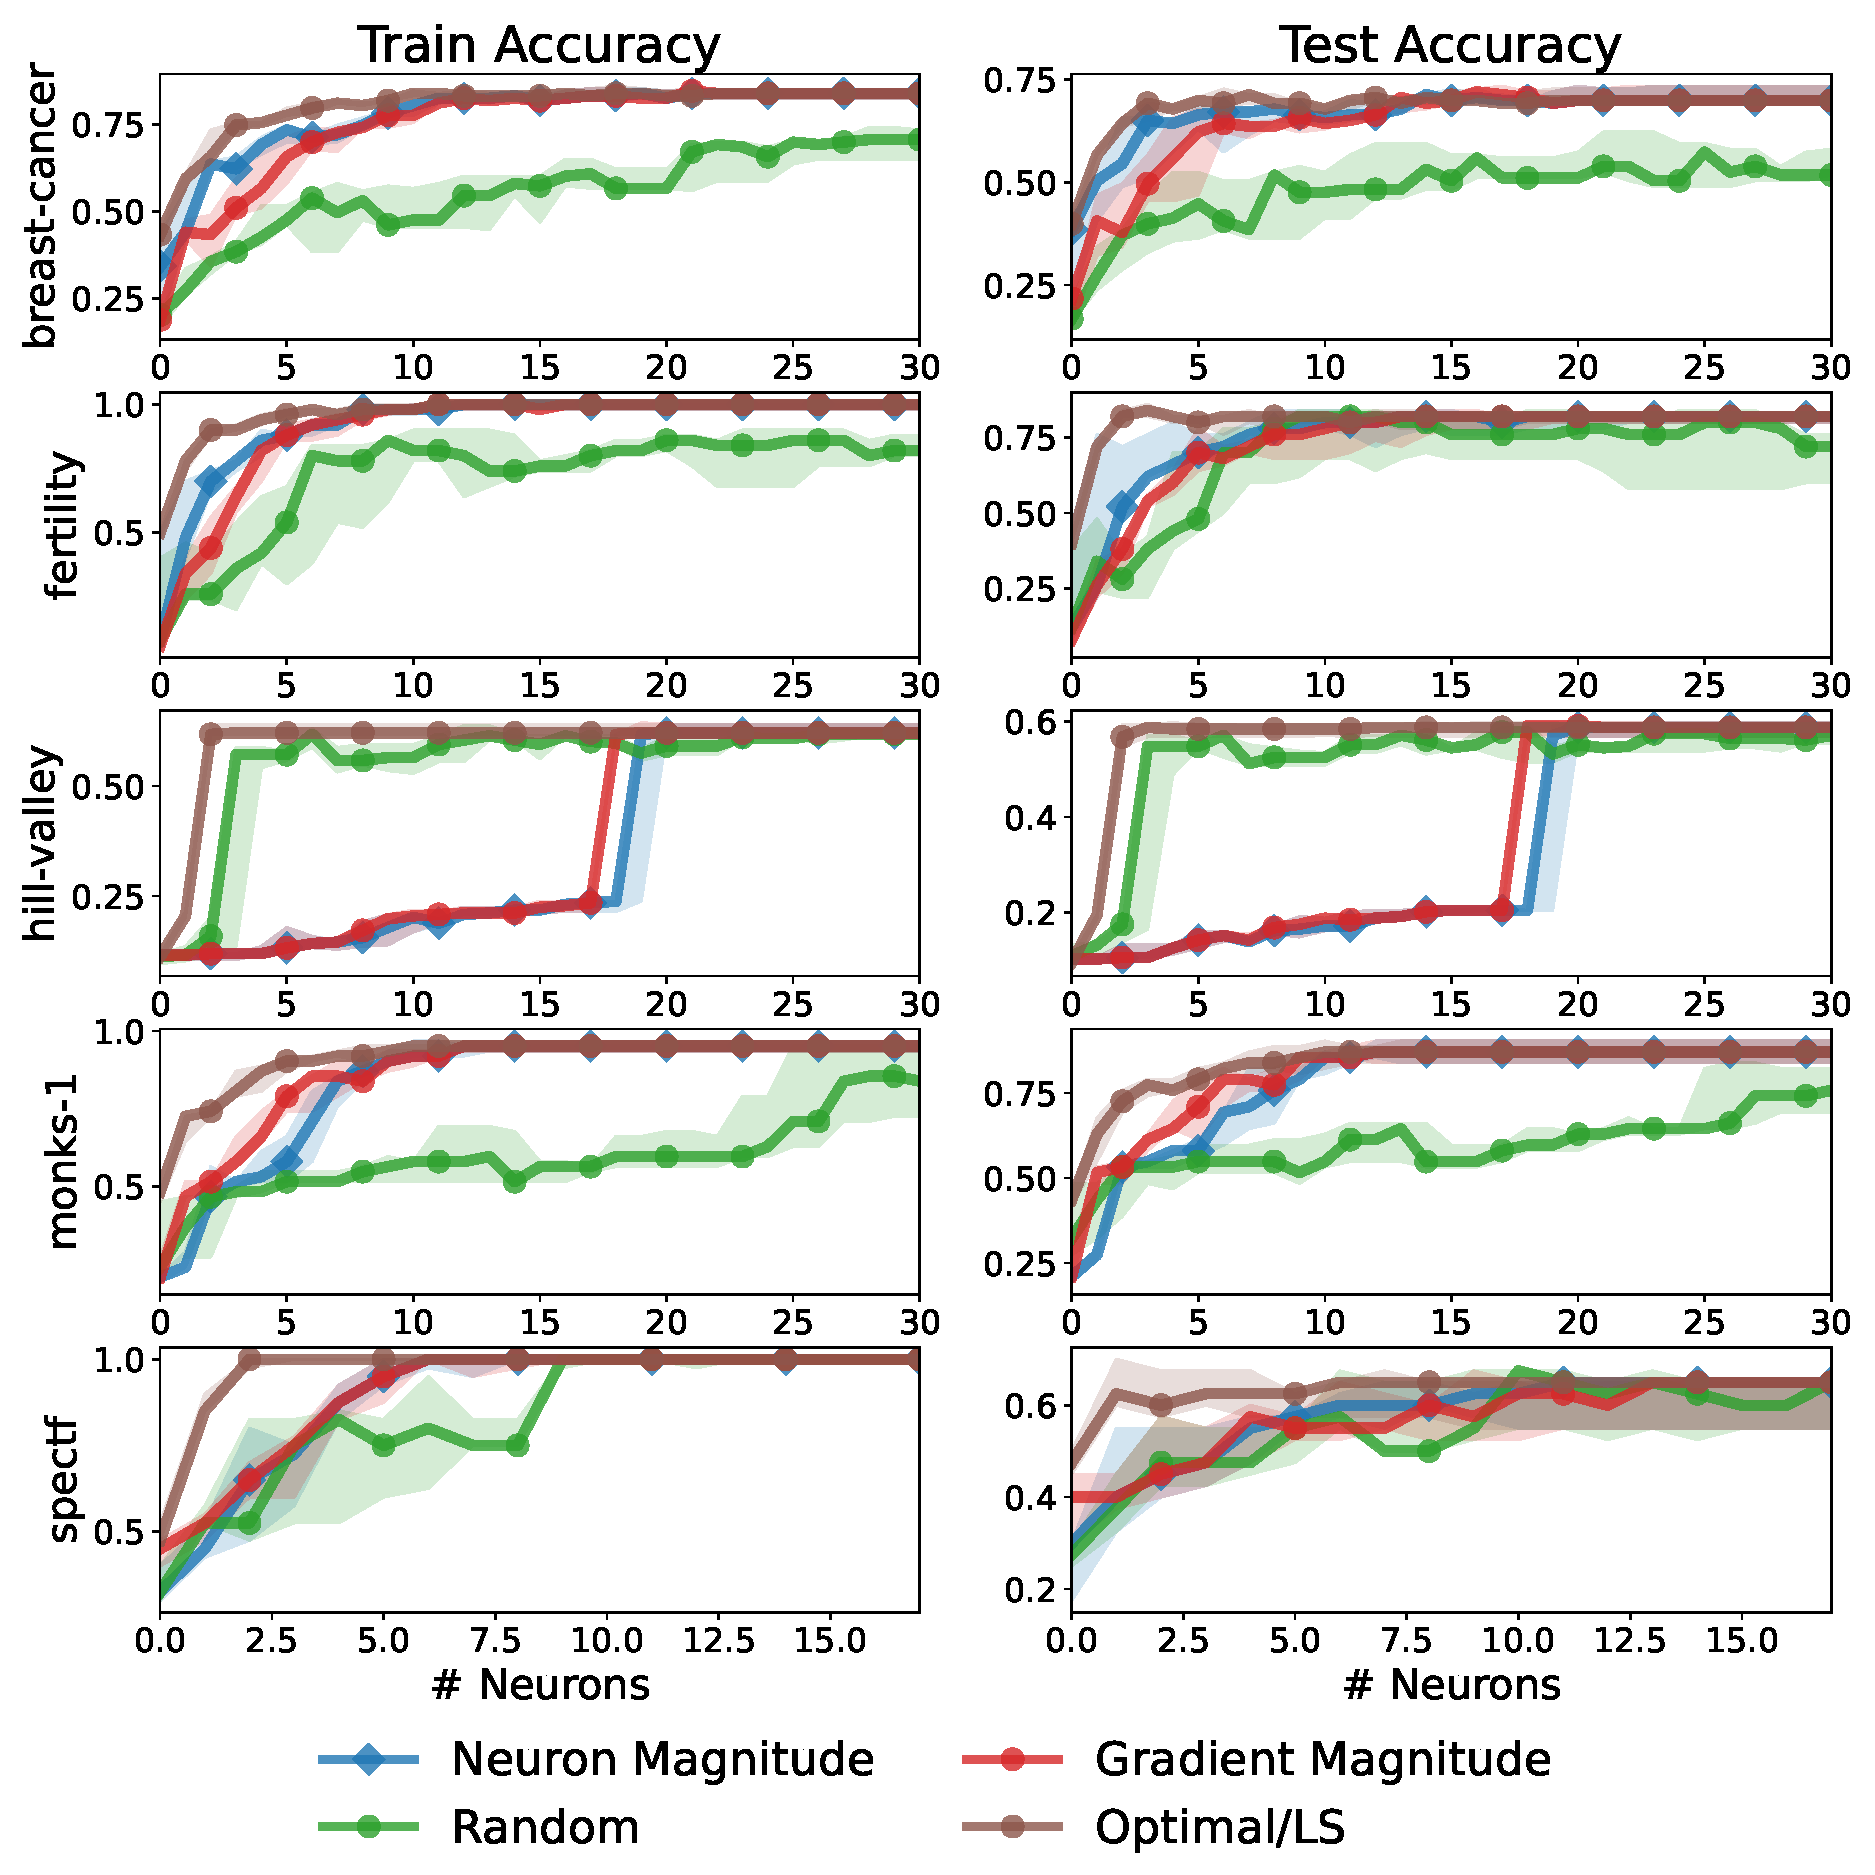
\includegraphics[width=0.75\textwidth]{assets/uci_pruning_full_paper.pdf}
	\end{figure}
\end{frame}

\begin{frame}{(Sub)-Optimal Pruning on CIFAR-10}
	\begin{figure}[t]
		\centering
		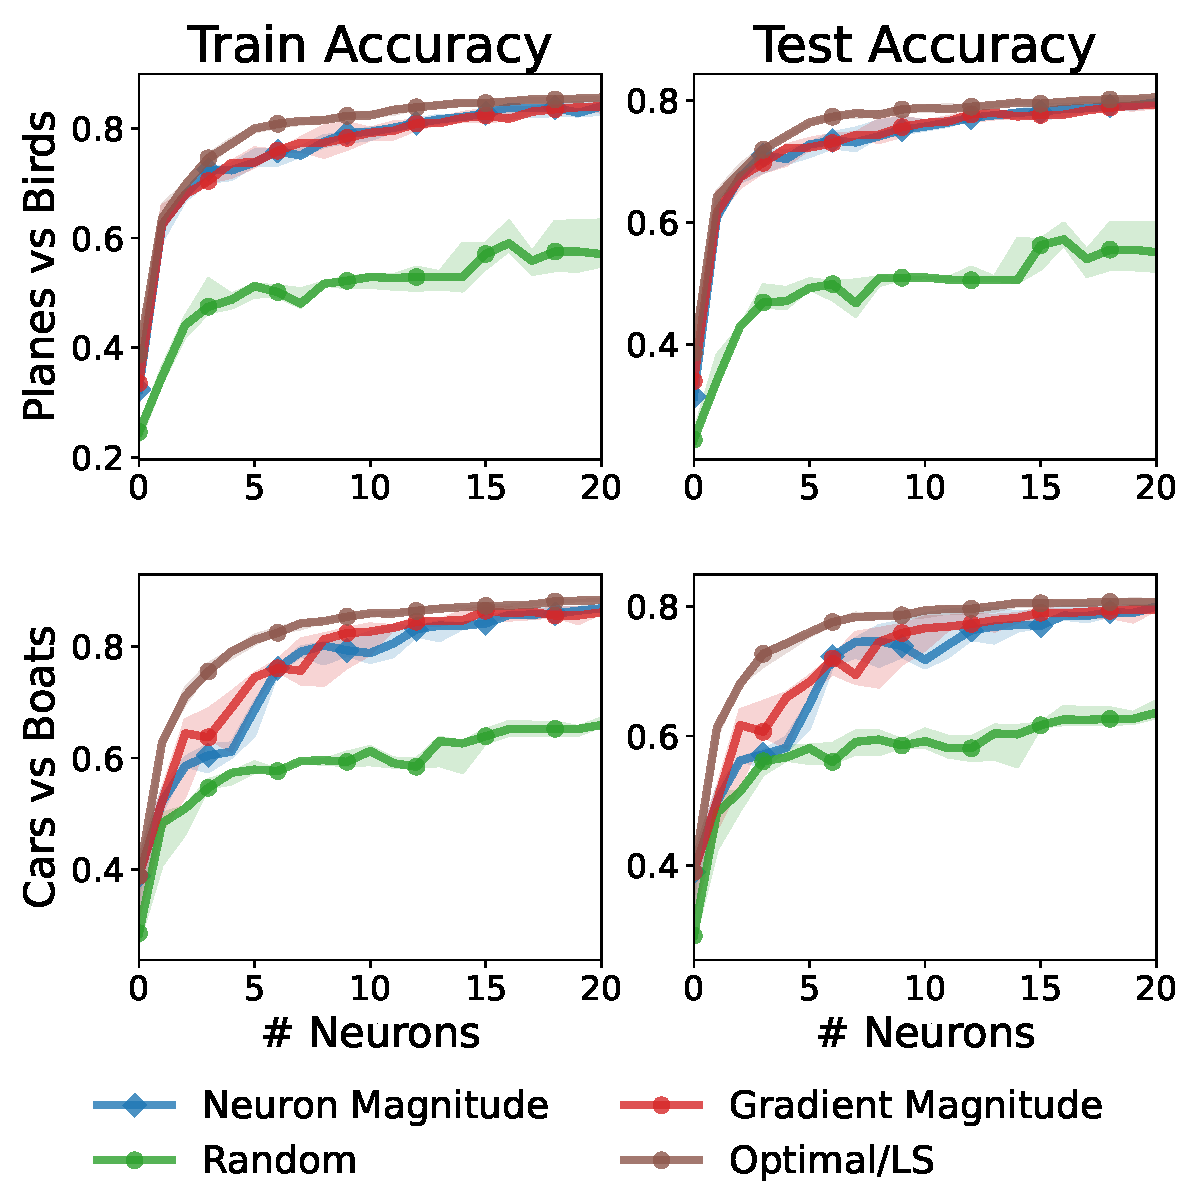
\includegraphics[width=0.75\textwidth]{assets/prune_cifar.pdf}
	\end{figure}
\end{frame}

\setbeamercolor{background canvas}{bg=LightCyan}

\begin{frame}{}
	\begin{center}
		\huge Pause.
	\end{center}
\end{frame}
\setbeamercolor{background canvas}{bg=white}

\begin{frame}{Recap}
	\begin{center}
		\huge   Our Contributions.
	\end{center}

	\vspace{2em}
	\pause
	{ \large
		\begin{itemize}
			\item \textbf{Optimal Sets}: We derive the set of all optimal
			      two-layer ReLU neural networks.
			      \pause
			      \vspace{0.5em}

			\item \textbf{Regularization Paths}: We have some continuity
			      results (see paper) and are working on more.
			      \pause
			      \vspace{0.5em}

			\item \textbf{Algorithms}: We give a poly-time algorithm for
			      optimally pruning ReLU networks.

		\end{itemize}
	}

\end{frame}


%% main content ends %%

%% end slide
\setbeamercolor{background canvas}{bg=LightCyan}

\begin{frame}{}
	\begin{center}
		\huge Try our Code!
	\end{center}

	\begin{figure}[]
		\centering
		
\includegraphics[width=0.6\textwidth]{assets/github.png}
	\end{figure}
\end{frame}
\setbeamercolor{background canvas}{bg=white}

%% bibliography
\begin{frame}[allowframebreaks]{References}
	\printbibliography[]
\end{frame}


\begin{frame}{Bonus: Explicit Optimal Set}
	We gave a characterization of \( \solfn(\lambda) \) that depends on
	\[
		\calS_\lambda
		= \cbr{\bi \in [2p] : \exists \theta \in \solfn(\lambda), \
			\theta_i \neq 0}.
	\]

	Alternative expression involves additional linear constraints.

	\pause
	\horizontalrule

	\begin{equation*}
		\begin{aligned}
			\solfn(\lambda) =
			\big\{ & \theta  :
			\forall \, \bi  \in  \equi,
			\theta_i =  \alpha_\bi q_i, \alpha_\bi \geq 0, \,           \\
			       & \quad \forall \, j \in [2p] \setminus \equi,
			\theta_{j} = 0, \, \sum_{i=1}^{2p} D_i X \theta_i = \hat y, \\
			       & \quad \forall \, i \in [2p],
			K_i \theta_i \geq 0, \abr{\rho, K_i \theta_i } = 0.
			\big\}
		\end{aligned}
	\end{equation*}

	\pause

	More complex, but also \textbf{explicit}.

\end{frame}

\begin{frame}{Bonus: Solution Mapping for C-ReLU}

	Given \( \rbr{v^*, w^*} \), an optimal non-convex ReLU network is given by

	\begin{equation*}
		\textbf{C to NC:} \quad \quad
		\begin{aligned}
			W_{1i} & = v_i^*/ \sqrt{\norm{v_i^*}}, \quad w_{2i} = \sqrt{\norm{v_i^*}}
			\\
			W_{1j} & = w_i^*/ \sqrt{\norm{w_i^*}}, \quad w_{2j} = -\sqrt{\norm{w_i^*}}.
		\end{aligned}
	\end{equation*}

	\pause
	\vspace{3ex}
	\begin{itemize}
		\item Optimal convex weights satisfy \( v_i^* = \alpha_i q_i \)
		      so that
		      \[
			      \norm{v_i^*}_2 = \alpha_i \norm{q_i}_2 = \alpha_i \lambda.
		      \]
	\end{itemize}

	\pause
	\horizontalrule

	Recall structure of \textbf{non-convex optima}:

	\begin{equation*}
		\begin{aligned}
			\hspace{-0.5em} \calO_\lambda  = \,
			\big\{
			 & (W_1,  w_2) :
			\, f_{W_1, w_2}(X)  =  \hat y,                       \\
			 & \forall \, \bi  \in  \calS_\lambda,
			W_{1i} = (\sfrac{\alpha_{i}}{\lambda})^{\sfrac{1}{2}} q_i,
			w_{2i} = (\alpha_i \lambda)^{\sfrac{1}{2}},
			\alpha_i \geq 0                                      \\
			 & \forall \, \bi  \in [2p] \setminus \calS_\lambda,
			W_{1i} = 0, \, w_{2i} = 0
			\big\}.
		\end{aligned}
	\end{equation*}

\end{frame}

\end{document}
